% \documentclass[whitelogo, 11pt]{TUD-report2020}
\documentclass{TUD-report2020}

\usepackage[style=numeric,sorting=none,block=space]{biblatex}
\addbibresource{report.bib}

\usepackage{changes}

\usepackage[skins, breakable]{tcolorbox}
\usepackage{mathdots}
\usepackage{svg}
\usepackage{graphicx}
\usepackage{wrapfig}
\usepackage{subcaption}
\usepackage{float}
\usepackage{MnSymbol}
\usepackage[toc,page]{appendix}
\usepackage{tikz}
\usepackage{tikzscale}
\usetikzlibrary{calc}
\usetikzlibrary{fit}

\usepackage{listings}
% \usepackage{codestyle}
\usepackage{codestyle}
\usepackage{mathtools}
\usepackage{amsthm}
\usepackage{multirow}
\usepackage{colortbl}
\usepackage{hhline}

\usepackage{array}
\usepackage{microtype}
\usetikzlibrary{decorations.pathmorphing,decorations.markings,calc}

% For appendix B, the proofs
\newtheorem{theorem}{Theorem}
\newtheorem{lemma}[theorem]{Lemma}
\newtheorem{definition}[theorem]{Definition}
\newcommand{\setminusD}{\mathbin{\backslash}}

% footnote without marker (in preface)
\newcommand\blfootnote[1]{%
  \begingroup
  \renewcommand\thefootnote{}\footnote{#1}%
  \addtocounter{footnote}{-1}%
  \endgroup
}

% For scaling equation that are too large
\newcommand\scalemath[2]{\scalebox{#1}{\mbox{\ensuremath{\displaystyle #2}}}}

% Antidiagonal dots
\DeclareRobustCommand{\Rdots}{\reflectbox{$\ddots$}}
% \newcommand{\addpage}{
%     \clearpage
%     \thispagestyle{empty}
%     \vspace*{\fill}
%     \newpage
% }

%% Hyperlinks are cyan.
\hypersetup{
    colorlinks=true,
    citecolor=title,
    linkcolor=title,
    urlcolor=title
}

\begin{document}
\renewcommand\UrlFont{\color{tudelft-cyan}\ttfamily}
\newcommand\Chapter[2]{
  \chapter[#1: {\itshape#2}]{#1\\[0ex]\Large\itshape#2}
}


%% Use Roman numerals for the page numbers of the title pages and table of
%% contents.
\frontmatter

\title[tudelft-black]{Methods for reducing error in approximations of the Rayleigh integral}
\author[tudelft-white]{Joris Perrenet}
\coverimage{pictures/real_3d_part_projected}
\covertext[tudelft-white]{
    \textbf{Bachelor Thesis 2022}
}

\makecover




%% Include an optional title page.
\begin{titlepage}


\begin{center}

%% Insert the TU Delft logo at the bottom of the page.

%% Print the title in cyan.
{\makeatletter
\fontsize{40}{40}\selectfont\@title
%\largetitlestyle\color{tudelft-cyan}\Huge\@title
\makeatother}

%% Print the optional subtitle in black.
{\makeatletter
\ifx\@subtitle\undefined\else
    \bigskip
   {\tudsffamily\fontsize{22}{32}\selectfont\@subtitle}
    %\titlefont\titleshape\LARGE\@subtitle
\fi
\makeatother}

\bigskip
\bigskip

by

\bigskip
\bigskip

%% Print the name of the author.
{\makeatletter
\fontsize{30}{30}\selectfont\@author
\makeatother}

\bigskip
\bigskip

to obtain the degree of Bachelor of Science in

Applied Mathematics and Applied Physics

at the Delft University of Technology,

to be defended publicly on Friday, 1 July, 2022 at 14:00.

\vfill

\begin{tabular}{lll}
    Student number: & 5293243 \\
    Project duration: & \multicolumn{2}{l}{24 February 2022 -- 1 July 2022} \\
    Thesis committee: & Prof.\ dr.\ ir.\ C.\ Vuik, & TU Delft, EWI supervisor \\
        & Dr.\ ir.\ D.\ J.\ Verschuur, & TU Delft, TNW supervisor \\
        & Dr.\ ir.\ Y.\ M.\ Dijkstra, & TU Delft, EWI \\
        & Dr.\ W.\ A.\ van Dongen, & TU Delft, TNW \\
    Additional supervision: & Ir. L.A. Hoogerbrugge, & TU Delft, TNW \\
\end{tabular}
%% Only include the following lines if confidentiality is applicable.

\bigskip
\bigskip
\bigskip
\bigskip
An electronic version of this thesis is available at \url{http://repository.tudelft.nl/}.

% The uncompiled, \LaTeX version is available at \url{https://github.com/jorisperrenet/BachelorThesis}.
An uncompiled, \LaTeX\ version of this thesis is available at \url{https://github.com/jorisperrenet/BachelorThesis}.
%\\[1cm]

\end{center}

\begin{tikzpicture}[remember picture, overlay]
    \node at (current page.south)[anchor=south,inner sep=0pt]{
        % \includegraphics{cover/logo_black}
        \includegraphics{cover/logo}
    };
\end{tikzpicture}

\end{titlepage}



\chapter*{Preface}
\setheader{Preface}
\addcontentsline{toc}{chapter}{Preface}

You are currently reading the thesis ``\makeatletter\@title\makeatother''. It has been written in order to obtain the degree of Bachelor of Science in Applied Mathematics and Applied Physics at the Delft University of Technology. I engaged in researching and writing this thesis from the 24th of February to the 1st of July in the year 2022.

From a young age I was captivated by prime numbers. At first, I studied them on paper, but through lack of brain power I started to write computer code. As I got older the efficiency of my computer code increased and from it originated my fascination for programming and optimizing algorithms.
Researching and enhancing the calculation of the Rayleigh integral using my knowledge obtained inside and outside this Bachelor degree was therefore an interesting quest and a joyful challenge.

I would like to thank my supervisors, Kees Vuik and Eric Verschuur, as they were of great help during my bachelor thesis. I was especially thankful for the freedom they gave me to explore the topics I found appealing, whilst making sure that the topics remained relevant for present-day applications.
I am also grateful for Yoeri Dijkstra and Koen van Dongen, the other members of my thesis committee, for attending the defense of my thesis and assessing this report.
In addition, Leo Hoogerbrugge, currently Eric's PhD-student, provided great knowledge and assistance in our weekly meetings.

Further gratitude goes out towards my parents, my brothers, and friends. The feedback I received about the content, code and layout of this thesis was very helpful and more than appreciated.

\begin{flushright}
{\makeatletter\itshape
    \@author \\
    The Hague, July 2022
\makeatother}
\end{flushright}

\blfootnote{The figure at the cover is Figure \ref{fig:real_3d_projected_wavefield}, displaying an artificial integrand of the Rayleigh integral. In this thesis we develop various methods to integrate this function, which we then compare at the end.}

\chapter*{Abstract}
\setheader{Abstract}
\addcontentsline{toc}{chapter}{Abstract}
The goal of seismic imaging is to create a model of the subsurface from samples of a transmitted wavefield that is reflected in soil layers.
The created model can be used to locate storage possibilities for CO$_2$ or H$_2$ or to find oil and gas reservoirs or other natural resources.
Seismic imaging relies on the propagation of wavefields, which can be computed by evaluating the Rayleigh integral, a process that often requires a lot of time and resources.
In this thesis we develop methods to reduce error in the computation of the Rayleigh integral whilst remaining time-efficient.
To achieve this we first give the derivation of the Rayleigh integral and provide a few methods to evaluate integrals numerically using interpolating polynomials.
Afterwards, we adapt the integration methods to the Rayleigh integral and arrive at the main algorithms for its evaluation, at the end we compare these algorithms.

We present the method that is currently used for the computation of the Rayleigh integral and a modification that extends the method to samples on a rectilinear grid.
The adjusted version of this method did not perform consistently in our results, although it achieved better results than the original method on average.
Secondly we present a combined interpolation method (that is, it interpolates the full integrand without taking advantage that one of the two functions in the integrand is known) named Simpson's rule, which only performed better in the high sample points per wavelength range with minimal noise.
An alteration to the method for semi-equidistant grids (see Section \ref{doub_alter} for the definition) also did not perform consistently and is not worth the extra operations.
Next was the separate interpolation algorithm (this time taking advantage of the known part of the integrand), this method is difficult to implement and had only slightly better performance than the combined method.
The final method was an extension of the separate interpolation algorithm to non-equidistant grids, this method performed undoubtedly the best of all presented methods (often better by a factor of 15 compared to the currently used method), this method is therefore recommended for evaluating the Rayleigh integral.
The amount of operations needed for all presented methods is approximately the same and the execution time needed for the calculation depends on the implementation of the problem.

In conclusion, we found that the separate interpolation method for non-equidistant grids delivered the most accurate approximations of the Rayleigh integral. This method can be used in seismic imaging to increase the accuracy of models of the subsurface.


{
    % \newgeometry{hscale=0.75,vscale=1}
    % \fontsize{11.5}{12}\selectfont
    \microtypesetup{protrusion=false}
    \hypersetup{linkcolor=black}
    \tableofcontents
}

%% Use Arabic numerals for the page numbers of the chapters.
\mainmatter

\chapter{Introduction}
Imagine you are walking down the beach, and you look at the horizon.
An oil drilling platform crosses your sight, and you suddenly start to wonder;
how do oil companies know where to drill? How do they know that the drilling platform must be placed at exactly that spot?
The answer lies in using (marine) seismic imaging, a technique based on wavefield propagation, to produce an image of the subsurface.
Using such images it is possible to find storage possibilities for CO$_2$ or H$_2$ or to locate reservoirs that contain oil and gas or other natural resources.

\section{Problem description}
\begin{wrapfigure}{r}{0.5\textwidth}
    \vspace{-3.3em}
    \centering
    \includegraphics[width=0.5\textwidth]{pictures/seismic_acquisition}
    \caption{Simplified version of marine seismic acquisition to find a potential storage space for CO$_2$. Different properties of soil layers are denoted by different shades of brown. Often the source and the receivers are towed by a survey ship moving with a constant speed to increase the amount of data, also, the source is usually located in the midst of the receivers.}
    \label{fig:sea_floor}
    \vspace{-0.8em}
\end{wrapfigure}
In Figure \ref{fig:sea_floor} we display a simplified version of marine seismic imaging.
A source, typically an air gun at sea, transmits a wavefield close to the surface.
A fraction of the transmitted wavefield propagates through the different layers of soil (in the figure this is displayed using arrows) and only a small part of the emitted wavefield is reflected in just the right way to be picked up by the receivers.
Data processing then allows us to reconstruct a model of the subsurface by propagating the wavefield backwards, that is, from the collected data at the receivers we try to trace back the path that the waves took.
Specifically, if we assume that the layers extend horizontally, the Rayleigh integral describes the propagation of a wavefield from one layer to the next.
The assumption of horizontal layers is often an acceptable loss as methods without this assumption are overly complicated.
In order to obtain knowledge of the different structural layers of the subsurface it is required to evaluate this integral multiple times for each layer (as waves can get reflected many times).

This brings us to the problem: evaluating the Rayleigh integral takes a lot of time and requires a lot of computing power, as it needs to be done many times and the integral itself is difficult to compute.
Also, because the wavefield is propagated numerous times through all the layers of the subsurface, a small mistake in the beginning can amplify errors at the end.
This leads us to the main research question of this thesis:
\begin{tcolorbox}[enhanced, size=fbox, shadow={2.1mm}{-2mm}{0mm}{gray!20!white}, boxrule={.5pt}, colback=white, boxsep=10pt, left=5pt, right=5pt, sharp corners]
    \textsc{Research objective} \\
    To find an algorithm that reduces error in the evaluation of the Rayleigh integral compared to existing and currently used methods whilst maintaining (or lowering) the time complexity.
\end{tcolorbox}

\section{Thesis outline}
To achieve our objective and explain our results, this thesis contains the following chapters:
\begin{itemize}
    \item Chapter \ref{chap2}: \textsl{Deriving the Rayleigh integral}. This chapter contains the derivation of the Rayleigh integral. In order to derive the integral we must first derive the acoustical wave equation. This is done by combining relations from Hooke's law and Newton's law. Afterwards we transform the wave equation into the Helmholtz equation, which we then solve by using contour integration. From the solution we derive two main results: the wavefield of a point-source and the wavefield of a point-sink. A seeming paradox that there are multiple solutions to the same equation is explained further in Section \ref{solving_helmholtz}. Using our previous results we can then derive the Kirchhoff integral, the predecessor of the Rayleigh integral. By making an assumption and using a mathematical trick developed by Rayleigh we can then derive the Rayleigh integral. The integral describes the propagation from one layer of soil to the next, which is of vital importance for seismic imaging. In following chapters we seek to find methods that can approximate the integral numerically.
    \item Chapter \ref{chap3}: \textsl{Numerical integration using interpolating polynomials}. In this chapter we propose two methods for approximating a simplified version of the Rayleigh integral. Both methods are based on interpolating the integrand by polynomials. The first method makes use of a known part of the integrand (the integrand is a product of two functions, one of which is known) and the second method does not. The first method is however more difficult to implement than the second method as it differs greatly from currently used methods. In the final section of this chapter we provide numerical examples that use both methods to approximate an integral. The corresponding computer code can be found in Appendix \ref{app:code}. Both methods lay the groundwork for other methods we derive in the next chapter. The focus of our thesis is to compare both methods (and all methods that originate from them) to the currently used method.
    \item Chapter \ref{chap4}: \textsl{Adapting numerical integration methods for the Rayleigh integral}. In this chapter we get rid of the simplified version of the Rayleigh integral and translate the developed methods to fit the Rayleigh integral. An assumption made in the previous chapter, one that the receivers are placed exactly equidistant, is weakened. In the last section we provide a summary of all the derived methods. This is important because in the next chapter (Chapter \ref{chap5}) we compare the methods to the one currently used. We note that by using all the derived methods we can better approximate the Rayleigh integral, which can in turn be useful for seismic imaging, leading to lower error in models that can support drilling decisions.
    \item Chapter \ref{chap5}: \textsl{Results}. This chapter contains the results of the derived methods applied to synthetically constructed data, similar to the actual Rayleigh integral. At the end of this chapter we give a comparison of the performance of the methods and compare them to the method that is currently used. Inconsistencies in the methods are also discussed by comparing averaged data to single data. This chapter provides the foundation for the conclusion (Chapter \ref{conclusion}) and lists the key results from this thesis.
    \item Chapter \ref{conclusion}: \textsl{Conclusion and outlook}. In this chapter the main results of our thesis combined with a short introduction of the problem are given. At the end, we lay out subjects for future research, both theoretical and experimental.
    \item Appendices: In \textsl{Appendix \ref{appendix:wave_eq}} we discuss a verification of the acoustic wave equation derived in Chapter \ref{chap2}, the verification is more intuitive than the one given and provides support for the correctness of the other derivation. In \textsl{Appendix \ref{app:proofs}} we provide proofs for various statements in Subsection \ref{sec:cotesian}. \textsl{Appendix \ref{app:B}} contains the matrices used in the numerical examples in Section \ref{examples}, whereas \textsl{Appendix \ref{app:code}} contains the computer code used to generate the examples. This appendix also contains the computer code for the results (Chapter \ref{chap5}).
\end{itemize}

\section{Preliminaries and notational conventions}
In this section we provide the notational conventions that are used throughout this thesis.
Also, we provide a few Fourier transformations (including the definition) that function as lemmas for further derivations.

\subsection*{Notation}
In general, vectors are three-dimensional and denoted by a \textbf{bold} letter, i.e. $\mathbf v = (v_x, v_y, v_z)^\top$ is a vector whereas $\omega$ is not.
Also, we define $\mathbf r$ to be the position vector, thus $\mathbf r = (x, y, z)^\top = x\mathbf{\hat x} + y\mathbf {\hat y} + z\mathbf{\hat z}$ where $\mathbf{\hat x}$, $\mathbf{\hat y}$, and $\mathbf{\hat z}$ denote the unit vectors in the $x$, $y$, and $z$-directions, respectively.

Using the same unit vectors we define the gradient of a scalar field $f$ as:
\begin{equation}
    \nabla f \coloneq \mathbf{\hat x} \frac{\partial f}{\partial x} + \mathbf{\hat y} \frac{\partial f}{\partial y} + \mathbf{\hat z} \frac{\partial f}{\partial z} \,. \nonumber
\end{equation}
Note that $(\partial/\partial x)$ is used to denote the derivative in the $x$-directions and similar notations are used for the $y$ and $z$-directions.
The Laplacian of a scalar field $f$ is given as:
\begin{equation}
    \nabla^2 f \coloneq \mathbf{\hat x} \frac{\partial^2 f}{\partial x^2} + \mathbf{\hat y} \frac{\partial^2 f}{\partial y^2} + \mathbf{\hat z} \frac{\partial^2 f}{\partial z^2} \,. \nonumber
\end{equation}
For more information on the gradient or the Laplacian of a scalar field we refer the reader to \citeauthor{electrodynamics} \cite[Sections 1.2.3-1.2.7]{electrodynamics}.

The Dirac delta function is defined by the following two equations:
\begin{equation}
    \delta(x) \coloneq \begin{cases} 0 & \textrm{if } x\neq 0\\ \infty & \textrm{if } x=0\end{cases} \,, \quad
    \int_{-\infty}^\infty \delta(x) \mathrm d x = 1 \,. \nonumber
\end{equation}
In three dimensions this definition extends to
\begin{equation}
    \delta(\mathbf r) \coloneq \delta(x) \delta(y) \delta(z) \,. \nonumber
\end{equation}
Again, for more information the reader is referred to \citeauthor{electrodynamics} \cite[Sections 1.5.1-1.5.3]{electrodynamics}.

We use big $\mathcal O$ notation (also known as Bachmann-Landau notation or asymptotic notation) to denote the time and space complexity of our algorithms.
Below, we give the formal definition, for more information the reader is referred to \citeauthor{bigOnotation} \cite[Section 4.3]{bigOnotation}.
\begin{tcolorbox}[sharp corners, colback=white]
    Let both $f(n)$ and $g(n)$ be real valued functions. Then $f(n)$ is $\mathcal O(g(n))$ if there is a real constant $c>0$ and a real number $n_0$ such that:
    \begin{equation}
        f(n) \leq c \cdot g(n) \,, \quad \textrm{for} \quad n \geq n_0 \,. \nonumber
    \end{equation}
\end{tcolorbox}

We note that notations that are not specified above are defined when they are used.

\subsection*{Fourier transformations}
In this subsection we provide a few Fourier transformations together with the definition, we note that the spatial variant and the temporal variant are both used in this thesis.
In order to signify that we use a spatial Fourier transform we denote the spatial transformation with $\mathcal F \{ \dots \}(\mathbf q)$.
The three-dimensional spatial Fourier transformation is defined as \cite[Section 3.4]{Fourier_transform}:
\begin{equation}
    \mathcal F\{u\}(\mathbf q) = \frac{1}{(2\pi)^3} \int_{-\infty}^{\infty} u(\mathbf r) e^{-i \mathbf q \cdot \mathbf r} \mathrm d^3 \mathbf r \,,\label{eq:fourier_trans}
\end{equation}
\begin{equation}
    u(\mathbf r) = \int_{-\infty}^{\infty} U(\mathbf q) e^{i \mathbf q \cdot \mathbf r} \mathrm d^3 \mathbf q \,.\label{eq:inv_fourier}
\end{equation}
With these integrals we mean to denote the integration over all components of $\mathbf r$ (or $\mathbf q$) where each integral extends from $-\infty$ to $\infty$, also, $\mathbf q \cdot \mathbf r$ represents the dot product between $\mathbf q$ and $\mathbf r$, i.e. $\mathbf q \cdot \mathbf r = q_x r_x + q_y r_y + q_z r_z$.

For a temporal Fourier transformation we write a capital function letter, thus
\begin{equation}
    x(t) \stackrel{\mathcal F}{\longleftrightarrow} X(\omega) \,, \nonumber
\end{equation}
where we used $\stackrel{\mathcal F}{\longleftrightarrow}$ to mark a Fourier transformation.
The transformations are then given by \cite[equations 4.8 \& 4.9]{signals_and_systems}:
\begin{equation}
    X(\omega) \coloneq \int_{-\infty}^{\infty} x(t) e^{-i\omega t} \mathrm d t \,, \label{eq:temporal_fourier_transform}
\end{equation}
\begin{equation}
    x(t) \coloneq \frac{1}{2\pi} \int_{-\infty}^{\infty} X(\omega) e^{i\omega t} \mathrm d \omega \,. \label{eq:reverse_time_fourier}
\end{equation}

We also derive the spatial Fourier transformation of the Dirac delta function centered around $\mathbf 0$ (the origin), as we will use it in Section \ref{solving_helmholtz}:
\begin{align}
    \delta(\mathbf r) \stackrel{\mathcal F}{\longleftrightarrow} \mathcal F \{\delta\}(\mathbf q) &= \frac{1}{(2\pi)^3} \int_{-\infty}^\infty \delta(\mathbf r) e^{-i\mathbf q \cdot \mathbf r} \mathrm d^3 \mathbf r \nonumber \\
    &= \frac{1}{(2\pi)^3} e^{-i\mathbf q \cdot \mathbf 0} = \frac{1}{(2\pi)^3} \,. \label{eq:fourier_delta}
\end{align}


\subsubsection{(anti)causality}
For Section \ref{solving_helmholtz} we need to establish the definition of causality.
We define a system to be \textbf{causal} if the output of the system at any time solely depends on the values of the input at present or past times \cite[Section 1.6.3]{signals_and_systems}.
Similarly, a system is called \textbf{anticausal} if the output of the system at any time solely depends on the values of the input at present or future times.
Thus, the system $y(t) = x(t)$ is causal as well as anticausal, $y(t) = x(t-t_0)$ with $t_0 \geq 0$ is causal but not anticausal, and $y(t) = x(t^2)$ is neither causal nor anticausal.

Since Section \ref{solving_helmholtz} also uses the time shifting property of the temporal Fourier transform \cite[Section 4.3.2]{signals_and_systems} we derive the property here.
% Starting with equation \ref{eq:reverse_time_fourier} and replacing $t$ by $t-t_0$ gives:
We start with equation \ref{eq:reverse_time_fourier} and replace $t$ by $t-t_0$:
\begin{align}
    x(t-t_0) &= \int_{-\infty}^{\infty} X(\omega) e^{i\omega (t-t_0)} \mathrm d \omega \nonumber \\
             &= \int_{-\infty}^{\infty} \left[ e^{-i\omega t_0} X(\omega) \right] e^{i\omega t} \mathrm d \omega \,. \nonumber
\end{align}
We can thus see that
\begin{equation}
    x(t-t_0) \stackrel{\mathcal F}{\longleftrightarrow} e^{-i\omega t_0} X(\omega) \,. \label{eq:time_shift}
\end{equation}
We end this section by noting that in the frequency domain, if we multiply $X(\omega)$ (which in this case denotes the Fourier transform of an input that solely depends on the present) by a negative exponent (i.e. $e^{-i\omega t_0}$ with $t_0 \geq 0$), we get a causal function in the time domain and vice versa.
This will be important when we take on solving the Helmholtz equation in Section \ref{solving_helmholtz}.

\chapter{Deriving the Rayleigh integral}
\label{chap2}
In this chapter we derive the Rayleigh integral. Using this integral we can calculate the pressure wavefield at different depths in the subsurface, which is crucial for constructing a model of the subsurface.
% Such a model can in turn be useful for finding structures and abnormalities in Earth's layers, mainly used for finding storage possibilities for CO$_2$ and locating oil and gas reservoirs.

The derivation of the integral is rather long, however important, thus we devote this entire chapter to it.
Further information on the derivation can be found in \citeauthor{Book_Eric} \cite[Chapter 3-4]{Book_Eric} and in \citeauthor{Kutscha} \cite[Appendix A]{Kutscha}, which provided a basis for this chapter.

We start with deriving the three-dimensional acoustic wave equation, which translates to the Helmholtz equation in the frequency domain.
The Helmholtz equation is then solved, yielding two cardinal results: the wavefield of a point-source and the wavefield of a point-sink.
Afterwards we derive the Kirchhoff integral, which in combination with our previous results and a trick developed by Rayleigh allows us to derive the Rayleigh integral.

\section{Deriving the acoustic wave equation}
\label{sec:wave_eq}
In this section we derive the three-dimensional acoustic wave equation, since the derivation is rather algebraic we provide a more intuitive method for deriving the one-dimensional version in Appendix \ref{appendix:wave_eq}.
This can also be used as a verification of the algebraic approach.

\begin{wrapfigure}{r}{.5\textwidth}
    \vspace{-1.5em}
    \centering
    \includegraphics[width=.5\textwidth]{pictures/cube_vectors}
    \vspace{-2em}
    \caption{Infinitesimal volume element with dimensions $\Delta x$, $\Delta y$ and $\Delta z$, experiencing forces on its six faces due to excess pressure $p(\mathbf r, t)$.}
    \label{fig:cube}
    \vspace{-1em}
\end{wrapfigure}

We start off by considering an infinitesimal volume element with $\Delta V = \Delta x \Delta y \Delta z$, displayed in Figure \ref{fig:cube}, experiencing a total pressure $p_{tot}(\mathbf r, t)$ depending on position and time on each of its faces.

The total pressure consists of a static part $p_0(\mathbf r)$ independent of time and a time variant excess pressure part $p(\mathbf r, t)$:
\begin{equation}
    p_{tot}(\mathbf r, t) = p_0(\mathbf r) + p(\mathbf r, t) \,.\nonumber
\end{equation}
From now we only concern ourselves with the excess pressure field.

If there is such an excess pressure the volume element $\Delta V$ experiences displacement and deformation.
If the pressure on all six faces does not balance, the volume will experience a net force, causing it to accelerate.
We describe this by using Newton's (second) law.

However, we first look at the situation where the excess pressure does balance, this causes the volume element $\Delta V$ to undergo a change in volume due to confining pressure.
This change can be described by using Hooke's law.

After deriving relations describing the volume element by using Hooke's law and Newton's law we can combine the relations into the three-dimensional acoustic wave equation.
After solving the equation in the frequency domain we obtain the wavefield of a point-source and the wavefield of a point-sink.
These two equations lay the groundwork for the derivation of the Rayleigh integral.

\subsection{Hooke's law}
We start by writing out Hooke's law, which states that (relative) changes in the volume of a volume element due to confining pressure are proportional to that pressure (with a proportionality constant that can be space variant):
\begin{equation}
    p(\mathbf r, t) = -K(\mathbf r) \frac{\delta \Delta V}{\Delta V} \,, \label{eq:hook}
\end{equation}
where $\delta$ indicates a variation with time.
To get rid of the factor $\delta \Delta V / \Delta V$ we define the displacement vector field of the mass particles in the medium to be
\begin{equation}
    \mathbf u (\mathbf r, t) = \zeta(\mathbf r, t) \mathbf{\hat x} + \eta(\mathbf r, t) \mathbf{\hat y} + \xi(\mathbf r, t) \mathbf{\hat z} \,,\nonumber
\end{equation}
remembering that $\mathbf{\hat x}$, $\mathbf{\hat y}$, and $\mathbf{\hat z}$ denote the unit vectors in the $x$, $y$, and $z$-directions, respectively.
After writing $\Delta \zeta = \zeta(x+\Delta x) - \zeta(x)$ and defining $\Delta \eta$ and $\Delta \xi$ similarly, the increase in volume can now be written as
\begin{equation}
    \Delta V + \delta \Delta V = (\Delta x + \Delta \zeta) (\Delta y + \Delta \eta) (\Delta z + \Delta \xi) \,.\nonumber
\end{equation}
Bringing $\Delta V$ to the other side and writing out the right-hand side whilst omitting negligible factors (since $\Delta \zeta << \Delta x$, $\Delta \eta << \Delta y$, and $\Delta \xi << \Delta z$ for small variations in time we can neglect factors depending on products of these differences) gives us
\begin{equation}
    \delta \Delta V = (\Delta x \Delta y \Delta z - \Delta V) + \Delta x \Delta y \Delta \xi + \Delta x \Delta z \Delta \eta + \Delta y \Delta z \Delta \zeta \,.\nonumber
\end{equation}
Dividing by $\Delta V$ and taking the limit for small volume elements $\Delta V$ results in
\begin{equation}
    \lim_{\Delta V \to 0} \frac{\delta \Delta V}{\Delta V} = \frac{\partial \zeta (\mathbf r, t)}{\partial x} + \frac{\partial \eta (\mathbf r, t)}{\partial y} + \frac{\partial \xi (\mathbf r, t)}{\partial z} = \nabla \cdot \mathbf u (\mathbf r, t) \,.\nonumber
\end{equation}
This allows us to replace the factor $\delta \Delta V / \Delta V$ in Hooke's law (equation \ref{eq:hook}) by a component relating fields. This gives the equation
\begin{equation}
    p(\mathbf r, t) = -K(\mathbf r) \nabla \cdot \mathbf u(\mathbf r, t) \,.\nonumber
\end{equation}

Now, if we have a function $q(\mathbf r, t)$ describing the ``injected'' volume into the volume element (we previously did not take this into account) we can rewrite our previous equation into
\begin{equation}
    \nabla \cdot \mathbf u(\mathbf r, t) = -\frac{p(\mathbf r, t)}{K(\mathbf r)} + q(\mathbf r, t) \,. \label{eq:part1}
\end{equation}

\subsection{Newton's law}
Before deriving the three-dimensional acoustic wave equation we must acquire another relation using the displacement vector.
To do this, we use Newton's second law, it states that ``the change of motion of an object is proportional to the force impressed'' \cites[Section 6.2]{Book_Newton}[Section 1.1]{Book_Newton_2}.
Thus, if the forces on the volume element $\Delta V$ do not balance the volume element will experience acceleration, due to the element having mass and therefore inertia.
To put this into formulas, we work out the net force acting on the volume element in Figure \ref{fig:cube}:
\begin{align}
    \Delta F_x &= \Delta y \Delta z (p(x, y, z, t) - p(x+\Delta x, y, z, t)) \approx - \Delta x \Delta y \Delta z \frac{\partial p}{\partial x} \,,\nonumber \\
    \Delta F_y &= \Delta x \Delta z (p(x, y, z, t) - p(x, y+\Delta y, z, t)) \approx - \Delta x \Delta y \Delta z \frac{\partial p}{\partial y} \,,\nonumber \\
    \Delta F_z &= \Delta x \Delta y (p(x, y, z, t) - p(x, y, z+\Delta z, t)) \approx - \Delta x \Delta y \Delta z \frac{\partial p}{\partial z} \,.\nonumber
\end{align}
This can be rewritten as
\begin{equation}
    \Delta \mathbf F = - \Delta V \nabla p(\mathbf r, t) = \Delta m \mathbf a \,, \nonumber
\end{equation}
where it can be noted that the last equality follows from Newton's second law and that $\Delta m$ denotes the mass of the volume element (which can be written as $\rho \Delta V$, where $\rho$ denotes the space variant mass density).
After dividing by $\Delta V$, this yields
\begin{equation}
    - \nabla p (\mathbf r, t) = \rho(\mathbf r) \frac{\partial^2 \mathbf u(\mathbf r, t)}{\partial t^2} \,.\nonumber
\end{equation}

If we now add an external source $\mathbf f(\mathbf r, t)$ we get extra forces on the volume element, which results in a change of the previous formula, we obtain
\begin{equation}
    \mathbf f(\mathbf r, t)- \nabla p (\mathbf r, t) = \rho(\mathbf r) \frac{\partial^2 \mathbf u(\mathbf r, t)}{\partial t^2} \,. \label{eq:newton}
\end{equation}

\subsection{Combining the two results}
In this subsection we combine our results from Hooke's law and Newton's law into the three-dimensional acoustic wave equation.

To bring this about, we continue with equation \ref{eq:newton}, take the divergence and divide by the mass density:
\begin{equation}
    \nabla \cdot \frac{\mathbf f(\mathbf r, t)}{\rho(\mathbf r)} - \nabla \cdot \left[ \frac{\nabla p (\mathbf r, t)}{\rho(\mathbf r)} \right] = \nabla \cdot \frac{\partial^2 \mathbf u(\mathbf r, t)}{\partial t^2} \,. \nonumber
\end{equation}
Taking the second time derivative of equation \ref{eq:part1} results in
\begin{equation}
    \nabla \cdot \frac{\partial^2 \mathbf u(\mathbf r, t)}{\partial t^2} = -\frac{1}{K(\mathbf r)}\frac{\partial^2 p(\mathbf r, t)}{\partial t^2} + \frac{\partial^2 q(\mathbf r, t)}{\partial t^2} \,. \nonumber
\end{equation}
If we now equate the previous two equations we obtain
\begin{equation}
    \nabla \cdot \frac{\mathbf f(\mathbf r, t)}{\rho(\mathbf r)} - \nabla \cdot \left[ \frac{\nabla p (\mathbf r, t)}{\rho(\mathbf r)} \right] =  -\frac{1}{K(\mathbf r)}\frac{\partial^2 p(\mathbf r, t)}{\partial t^2} + \frac{\partial^2 q(\mathbf r, t)}{\partial t^2} \,. \label{eq:equated}
\end{equation}
In order to rewrite this equation we define
\begin{equation}
    s(\mathbf r, t) \coloneq \frac{\partial^2 q(\mathbf r, t)}{\partial t^2} - \nabla \cdot \frac{\mathbf f(\mathbf r, t)}{\rho(\mathbf r)}\,. \nonumber
\end{equation}
After substituting the new definition into equation \ref{eq:equated} and reorganizing we get
\begin{equation}
    \nabla \cdot \left[ \frac{\nabla p (\mathbf r, t)}{\rho(\mathbf r)} \right] - \frac{1}{K(\mathbf r)}\frac{\partial^2 p(\mathbf r, t)}{\partial t^2} = - s(\mathbf r, t) \,.\nonumber
\end{equation}

If we consider a homogeneous medium, $\rho$ and $K$ will no longer be space variant, yielding the relation
\begin{equation}
    \nabla^2 p (\mathbf r, t) - \frac{1}{c^2} \frac{\partial^2 p (\mathbf r, t)}{\partial t^2} = -s(\mathbf r, t) \,,\label{eq:helmholtz}
\end{equation}
with $c = \sqrt{K/\rho}$.
This is the three-dimensional acoustic wave equation (for homogeneous media), an important result as we will solve this equation in the frequency domain in the next section. Afterwards, we use the solutions to specify a known part of the Rayleigh integral.

\section{Wavefield of a single point-source}
In this section we continue with the acoustic wave equation derived in the previous section (Section \ref{sec:wave_eq}).
First, we transfer it to the frequency domain giving the Helmholtz equation, which we solve by deriving its Green's functions in the coming subsection (Subsection \ref{solving_helmholtz}).
The result corresponds to a known part of the Rayleigh integral, this part is crucial to derive as some developed integration methods make use of this.

Taking the three-dimensional acoustic wave equation (equation \ref{eq:helmholtz}) and substituting $-s(\mathbf r, t)$ with a single point-source at $\mathbf r_s$, whilst assuming that the point-source sends out one delta pulse, gives
\begin{equation}
    \nabla^2 p (\mathbf r, t) - \frac{1}{c^2} \frac{\partial^2 p (\mathbf r, t)}{\partial t^2} = \delta(t) \delta(\mathbf r-\mathbf r_s) \,.\label{eq:time_domain_wave_eq}
\end{equation}
In order to rewrite this equation, we first note that taking the time derivative on both sides of the inverse Fourier transformation in equation \ref{eq:reverse_time_fourier} results in
\begin{equation}
    \frac{\partial x(t)}{\partial t} \stackrel{\mathcal F}{\longleftrightarrow} i \omega X(\omega) \,. \nonumber
\end{equation}
That is, temporal differentiation in the time domain results in multiplication with $i\omega$ in the frequency domain.
Also, the Fourier transform of a delta function can be derived from equation \ref{eq:temporal_fourier_transform}:
\begin{equation}
    \delta(t) \stackrel{\mathcal F}{\longleftrightarrow} \int_{-\infty}^{\infty} \delta(t) e^{-i\omega t} \mathrm d t = 1 \,. \nonumber
\end{equation}
Using these relations, the Fourier transform of equation \ref{eq:time_domain_wave_eq} can be evaluated in order to obtain the Helmholtz equation:
\begin{equation}
    \nabla^2 P (\mathbf r, \omega) + \frac{\omega^2}{c^2} P (\mathbf r, \omega) = \delta(\mathbf r - \mathbf r_s) \,.\label{eq:PDE_fourier}
\end{equation}
In the next subsection (Subsection \ref{solving_helmholtz}) we solve the above equation, however, to set an objective, we first give the wavefield of a point-source and the wavefield of a point-sink (both solutions to the equation):
\begin{equation}
    P_{src} (\mathbf r, \omega) = \frac{e^{-i \omega |\mathbf r - \mathbf r_s| / c}}{4 \pi |\mathbf r-\mathbf r_s|} \quad \textrm{and} \quad
    P_{snk} (\mathbf r, \omega) = \frac{e^{i \omega |\mathbf r - \mathbf r_s| / c}}{4 \pi |\mathbf r-\mathbf r_s|} \,. \label{eq:greens_function}
\end{equation}

\subsection{Solving the Helmholtz equation}
\label{solving_helmholtz}
In this subsection we prove the validity of equation \ref{eq:greens_function} (the equation for the wavefield of a point-source and a point-sink) by solving the Helmholtz equation (equation \ref{eq:PDE_fourier}).
The seeming paradox that both equations are solutions to the same equation is also resolved in this subsection.
The solutions to the equations are used again in Section \ref{sec:rayleigh} where we derive the Rayleigh integral.

We solve equation \ref{eq:PDE_fourier} by deriving its Green's functions.
Due to symmetry we know that any Green's function will only depend on its magnitude of the distance between $\mathbf r$ and $\mathbf r_s$.
Thus after denoting $\mathbf r - \mathbf r_s$ by $\mathbf d$, any Green's function will eventually only depend on $|\mathbf d|$.
For now, we define $k = \omega/c$ and after noting that we assume $k$ to be constant we rewrite the Helmholtz equation (equation \ref{eq:PDE_fourier}) as (we omit the dependency on $\omega$ to avoid confusion)
\begin{equation}
    (\nabla^2 + k^2) G(\mathbf d) = \delta(\mathbf d)\,.\nonumber
\end{equation}
% In the remainder of this block $\mathbf q$ (and the later introduced $q$) will solely be used to denote the spatial frequency when using a Fourier transform.
If we apply the spatial Fourier transform in equation \ref{eq:fourier_trans} to the newly rewritten Helmholtz equation and define $|\mathbf q|^2 = q_x^2 + q_y^2 + q_z^2$ (remember that the Fourier transform of a delta function is given by equation \ref{eq:fourier_delta}, the differentiation property is given by \citeauthor{Fourier_transform} \cite[Section 3.4.3]{Fourier_transform} and can be easily verified by taking the derivative of equation \ref{eq:fourier_trans}), we get
\begin{equation}
    (k^2 - |\mathbf q|^2) \mathcal F\{ G\} (\mathbf q) = \frac{1}{(2\pi)^3} \,. \nonumber
\end{equation}
Rewriting this equation and taking the inverse spatial Fourier transform from equation \ref{eq:inv_fourier} we obtain
\begin{equation}
    G(\mathbf d) = -\frac{1}{(2\pi)^3} \int_{-\infty}^\infty \frac{e^{i \mathbf q \cdot \mathbf d}}{|\mathbf q|^2-k^2} \mathrm d^3 \mathbf q \,,\label{eq:greens_on_d}
\end{equation}
which is of the form
\begin{equation}
    \int_{-\infty}^\infty f(q) e^{i \mathbf q \cdot \mathbf d} \mathrm d^3 \mathbf q \,, \nonumber
\end{equation}
where $q$ is used to denote the magnitude of $\mathbf q$, i.e. $|\mathbf q|$. Since $f(q)$ does not depend on the direction of $\mathbf q$, this is equivalent to
\begin{equation}
    \frac{4\pi}{R} \int_0^\infty q f(q) \sin(q R) \mathrm d q \,,\nonumber
\end{equation}
with $R = |\mathbf d| = |\mathbf r - \mathbf r_s|$. For the proof of this statement the reader is referred to \citeauthor{Barton} \cite[Appendix F]{Barton}.
Rewriting equation \ref{eq:greens_on_d} by using the equivalence from above gives us
\begin{equation}
    G(R) = -\frac{4 \pi}{(2\pi)^3 R} \int_0^\infty \frac{q}{q^2-k^2} \sin(q R) \mathrm d q \,.\nonumber
\end{equation}
Note that we expected that any Green's function would only depend on the magnitude of $\mathbf r - \mathbf r_s$ (i.e. the newly defined $R$), which is indeed the case.
Since the integrand is even, we write:
\begin{equation}
    G(R) = -\frac{4 \pi}{(2\pi)^3 2R} \int_{-\infty}^\infty \frac{q}{q^2-k^2} \sin(q R) \mathrm d q\,. \nonumber
\end{equation}
The sine function can be expressed as a linear combination of exponentials:
\begin{equation}
    \sin(q R) = \frac{e^{iq R} - e^{-iq R}}{2i} \,, \nonumber
\end{equation}
which after substitution results in the following relation for $G(R)$:
\begin{equation}
    G(R) = -\frac{4 \pi}{(2\pi)^3 4iR} \bigg[ \underbrace{\int_{-\infty}^\infty \frac{q e^{i q R}}{(q-k)(q+k)} \mathrm d q}_{I_1} - \underbrace{\int_{-\infty}^\infty \frac{q e^{-i q R}}{(q-k)(q+k)} \mathrm d q}_{I_2} \bigg] \,.\label{eq:greens_2}
\end{equation}
We wish to find the integrals $I_1$ and $I_2$.
First we note that after a substitution of $q' = -q$ in $I_2$ we get $-I_1$ (the intervals also change due to this substitution resulting in the final minus sign).
Thus, all Green's function satisfy
\begin{equation}
    G(R) = -\frac{4 \pi}{(2\pi)^3 2iR} I_1 = -\frac{1}{4\pi^2 i R} I_1  \,.\nonumber
\end{equation}
We note that different Green's functions originate from different values of $I_1$.
Its value is evaluated further by means of contour integration.

We use a contour in the complex $q$ plane. However, due to poles on the real $q$-axis we first add the term $+i\epsilon$ to $k$ and take the limit $\epsilon \to 0$:
\begin{equation}
    I_1 = \lim_{\epsilon \to 0} \int_{-\infty}^\infty \underbrace{\frac{z e^{i zR}}{(z-(k+i\epsilon))(z+(k+i\epsilon))}}_{f(z)} \mathrm d z \,. \label{eq:contour_I_1}
\end{equation}
We can now see that $f(z)$ has poles at $z=k+i\epsilon$ and $z=-k-i\epsilon$, therefore, we take a contour in the upper half-plane, denoted by $\mathcal C$.
To clarify; the contour consists of the interval $[-A,A]$ and the semicircle $C_A = \{ Ae^{i\theta} | \theta \in [0, \pi] \}$.
From the residue theorem we get
\begin{align}
    \int_{\mathcal C} f(z) \mathrm d z &= 2 \pi i \lim_{\epsilon \to 0} \left( \textrm{Res}_{z=k+i\epsilon} [f(z)]\right) \nonumber \\
                                       &= 2 \pi i \lim_{\epsilon \to 0} \frac{(k+i\epsilon)e^{i(k+i\epsilon)R}}{2(k+i\epsilon)} \nonumber \\
                                       &= \pi i e^{ikR} \,, \nonumber
\end{align}
yielding the relation
\begin{equation}
    I_1 + \int_{C_A} f(z) = \pi i e^{ikR} \,. \nonumber
\end{equation}
We now show that $\int_{C_A} f(z) \to 0$ as $A \to \infty$.
From Jordan's lemma \cite[Section 74]{complex_jordan} with $f(z) = e^{izR}g(z)$ where $z \in C_A$ and $R$ is strictly positive, we get
\begin{align}
    \left| \int_{C_A} f(z) \mathrm d z \right| &\leq \frac{\pi}{R} \max_{\theta \in [0, \pi]} |g(Ae^{i\theta})| \nonumber \\
                                               &= \frac{\pi}{R} \max_{\theta \in [0, \pi]} \left\lvert \frac{Ae^{i\theta}}{(Ae^{i\theta}-k)(Ae^{i\theta}+k)} \right\rvert \nonumber \\
                                               &= \frac{\pi}{R} \max_{\theta \in [0, \pi]}  \frac{A}{\left\lvert A^2e^{2i\theta}-k^2\right\rvert}  \nonumber \\
                                               &= \frac{\pi}{R} \frac{A}{A^2-k^2} \,. \nonumber
\end{align}
We can thus see that $\int_{C_A} f(z) \to 0$ as $A \to \infty$.
Hence we have $I_1 = \pi i e^{i k R}$.
Note that if $R=0$ we get $I_1=I_2$ in equation \ref{eq:greens_2} and due to $R$ being in the denominator we get $G(0) = \delta(0)$, in this case, we did not have to use contour integration.

In addition, the option to add $-i\epsilon$ instead of $+i\epsilon$ to $k$ in equation \ref{eq:contour_I_1} is also possible, for that matter, we could even choose to add $-i\epsilon$ to the first occurrence of $k$ and $+i\epsilon$ to the second or vice versa\footnote{We also could have chosen to evaluate $I_2$. To achieve this, one can take a contour in the lower half plane and apply an equivalent form of Jordan's lemma. This removes the minus sign in front of $G(R)$.}.
All these options correspond to a different propagator, yielding a different result to the integral \cite[Section 3.6]{griffel}.
If we add $-i\epsilon$ instead of $+i\epsilon$ we get a pole in $\mathcal C$ at $z=-k+i\epsilon$, after following the same steps as above we get the result $I_1 = \pi i e^{-ikR}$.
Since this results comes from the pole at $-k$ we denote it as $I_1^{-} = \pi i e^{-ikR}$ and the result from above as $I_1^{+} = \pi i e^{ikR}$.
The other two results (from adding $-i\epsilon$ and $+i\epsilon$ or $+i\epsilon$ and $-i\epsilon$) are $0$ and $2 \pi i \cos(kR)$, respectively (note that $0$ is a correct solution for $I_1$ since we divide by $R$, which gives $G(R)=\delta(R)$, a solution to equation \ref{eq:PDE_fourier}).
The selected option of adding $\pm i \epsilon$'s determines the corresponding physical interpretation \cite[Section 11.2.2]{zettili}.
For example, $I_1^{-}$ represents \textit{outgoing} spherical waves from $\mathbf r_s$ (causal), whereas $I_1^{+}$ represents \textit{incoming} spherical waves (anticausal).
Note that this is not the other way around because we are in the (temporal) frequency domain and an exponential in the frequency domain leads to a time shift in the time domain (equation \ref{eq:time_shift}, noting that $k=\omega/c$) \cite[Section 4.3]{Book_Eric}.
The other two results (or any different linear combination of $I_1^+$ and $I_1^-$) are hereafter not used, they do not have an important physical meaning for our purposes.
% For more information on this subject the reader is referred to \cites[Section 3.6]{griffel}[Section 11.2]{zettili}[Section 4.3]{Book_Eric}{Greens1, Greens0, Greens2, Greens3, Greens4, greens_function, Greens5}.
For more information on this subject the reader is referred to \cites[Section 3.6]{griffel}[Section 11.2]{zettili}[Section 4.3]{Book_Eric}{Greens1, Greens0, Greens2, Greens3, Greens4, Greens5}.

From combining these results we obtain the Green's functions (note that if $R=0$ we still have $G(0)=\delta(0)$, the same expression as we derived without contour integration)
\begin{align}
    G^\pm(R) &= -\frac{1}{4\pi^2 iR} (\pi i e^{\pm ikR}) \nonumber \\
             &= -\frac{e^{\pm ikR}}{4\pi R} \,. \nonumber
\end{align}
We have thus shown that
\begin{align}
    G^\pm(\mathbf r, \omega) = -\frac{e^{\pm i\omega |\mathbf r - \mathbf r_s|/c}}{4\pi |\mathbf r-\mathbf r_s|}
\end{align}
are Green's functions of the Helmholtz equation (equation \ref{eq:PDE_fourier}).
From this we define $P_{src} (\mathbf r, \omega) = -G^- (\mathbf r, \omega)$ because it represents outgoing spherical waves and
$P_{snk} (\mathbf r, \omega) = -G^+ (\mathbf r, \omega)$ because it represents incoming spherical waves (note that the minus sign in front of these definitions is chosen because of $-s(\mathbf r, t)$ in equation \ref{eq:helmholtz}).

\section{Deriving the Kirchhoff integral}
\begin{wrapfigure}{r}{0.3\textwidth}
    \centering
    \includegraphics[width=0.3\textwidth]{pictures/kirchhoff_surface}
    \caption{Surface $S$ enclosing a volume $V$ with normal vector $\protect\overrightarrow{\mathbf n}$ pointed outward (enclosing a source placed at $\mathbf r_s$).}
    \vspace{-1em}
    \label{fig:volume}
\end{wrapfigure}
After solving the Helmholtz equation we can derive an independent result; the Kirchhoff integral.
This is the last step before deriving the Rayleigh integral in Section \ref{sec:rayleigh}.

If we take the Fourier transform of the three-dimensional acoustic wave equation in the absence of sources, i.e. equation \ref{eq:helmholtz} with $s(\mathbf r, t)=0$, we get
\begin{equation}
    \nabla^2 P(\mathbf r, \omega) + \frac{\omega^2}{c^2} P(\mathbf r, \omega) = 0 \,. \label{eq:1}
\end{equation}
Writing down the same equation for a point-source at $\mathbf r_s$ located inside the volume $V$ displayed in Figure \ref{fig:volume} (which gives $-s(\mathbf r, t) = -\delta(t)\delta(\mathbf r - \mathbf r_s)$) while using $G$ to denote the causal Green's function from equation \ref{eq:greens_function} (i.e. $P_{src}$), we get
\begin{equation}
    \nabla^2 G(\mathbf r, \omega) + \frac{\omega^2}{c^2} G(\mathbf r, \omega) = -\delta(\mathbf r - \mathbf r_s) \,.\label{eq:2}
\end{equation}
Now, multiplying equation \ref{eq:1} with $-G(\mathbf r, \omega)$ and adding it to equation \ref{eq:2} multiplied by $P(\mathbf r, \omega)$ and afterwards integrating over the volume $V$, leads to
\begin{equation}
    \int_V P(\mathbf r, \omega) \nabla^2 G(\mathbf r, \omega) - G(\mathbf r, \omega) \nabla^2 P(\mathbf r, \omega) \mathrm dV = \int_V -P(\mathbf r, \omega) \delta(\mathbf r - \mathbf r_s) \mathrm d V = -P(\mathbf r_s, \omega) \,.\nonumber
\end{equation}
Now Green's theorem \cite[Section 1.3.4]{electrodynamics} gives the Kirchhoff integral
\begin{equation}
    P(\mathbf r_s, \omega) = - \oint_S [P(\mathbf r, \omega) \nabla G(\mathbf r, \omega) - G(\mathbf r, \omega) \nabla P(\mathbf r, \omega)] \cdot \overrightarrow{\mathbf n} \mathrm dS\,. \label{eq:kirchhoff}
\end{equation}

\section{Deriving the Rayleigh integral}
\label{sec:rayleigh}
\begin{wrapfigure}{r}{.4\textwidth}
    \vspace{-1.2em}
    \includegraphics[width=.4\textwidth]{pictures/rayleigh_surface}
    \vspace{-2em}
    \caption{All sources generating the wavefield $P$ are below the flat plane $S_0$ with radius $R$. The semisphere $S_1$ also has radius $R$ and we consider the case where $R \to \infty$. The normal vector of $S_0$, i.e. $\protect\overrightarrow{\mathbf{n}}$, is defined outward. The prediction point is denoted by $A$, which lies inside the volume $V$. The source point generated by $\Gamma$ is in $A'$, which is the mirror position of $A$ with respect to the plane $S_0$.}
    \label{fig:semisphere}
    \vspace{-1em}
\end{wrapfigure}
In this section we finally derive the Rayleigh integral, this is done by using a mathematical trick due to Rayleigh.
The integral describes the propagation from one layer of the subsurface to the next assuming that the layers extend horizontally, an important result for (marine) seismic imaging.

Rayleigh's main idea was that we can add a homogeneous solution $\Gamma(\mathbf r, \omega)$ of the partial differential equation \ref{eq:PDE_fourier} to the Green's function (an inhomogeneous solution) to obtain another solution of the differential equation. For the remainder of this section we denote $P$, $G$ and $\Gamma$ instead of $P(\mathbf r, \omega)$, $G(\mathbf r, \omega)$ and $\Gamma(\mathbf r, \omega)$, respectively, whenever the chance of confusion is low.

Causality of the Kirchhoff integral in equation \ref{eq:kirchhoff} tells us that the same integral holds if we go from a source point $\mathbf r_s$ to a prediction point $\mathbf r_A$ \cite[Section 4.3]{Book_Eric} (that is, instead of transmitting a wavefield in $\mathbf r_s$ we can also predict the wavefield in the same point, denoted by the prediction point $\mathbf r_A$). Combining the homogeneous solution $\Gamma$ with the abbreviated notation allows us to rewrite equation \ref{eq:kirchhoff} into
\begin{equation}
    P(\mathbf r_A, \omega) = - \oint_S [P \nabla (G + \Gamma) - (G + \Gamma) \nabla P] \cdot \overrightarrow{\mathbf n} \mathrm dS \,. \nonumber
\end{equation}
If we apply this integral to the situation displayed in Figure \ref{fig:semisphere}, we can replace $S$ by $S_0$ in the above integral.
This can be justified since as $R\to \infty$ the wavefield $P$ generated below $S_0$ can only propagate outward with respect to the surface $S_1$ and thus can not (causally) contribute to any knowledge of the wavefield in $A$.

The trick was to let the field $\Gamma$ be generated in $A'$.
If we let $G(\mathbf r_A, \mathbf r_{S_0}) = - \Gamma (\mathbf r_{A'}, \mathbf r_{S_0})$ everywhere on $S_0$ then $G$ and $\Gamma$ cancel each other on $S_0$ (if we assume that $S_0$ is indeed a flat plane).
This can be done by making $\Gamma$ a point sink whenever $G$ is a point-source.
Because the wavefields cancel each other, continuity gives that the normal components of their gradients must be equal on $S_0$, i.e. $\nabla G(\mathbf r_{S_0}) = \nabla \Gamma (\mathbf r_{S_0})$, which is perfect, as the integral can now be rewritten into:
\begin{equation}
    P(\mathbf r_A, \omega) = - 2\oint_{S_0} [P \nabla G] \cdot \overrightarrow{\mathbf n} \mathrm dS_0 \,.\nonumber
\end{equation}
If the surface $S_0$ is assumed to be in the $x$,$y$-plane we get $\nabla G \cdot \mathbf n = -\partial G / \partial z$ due to an outward pointing normal vector.
Hence, the integral becomes:
\begin{equation}
    P(\mathbf r_A, \omega) = 2\oint_{S_0} P \frac{\partial G}{\partial z} \mathrm dS_0 \,.\label{eq:pre_rayleigh}
\end{equation}
Remember that the (causal) Green's function is given by equation \ref{eq:greens_function}:
\begin{equation}
    G(\mathbf r_A, \mathbf r; \omega) = \frac{e^{-i\omega |\mathbf r-\mathbf r_A|/c}}{4 \pi |\mathbf r- \mathbf r_A|} \,. \nonumber
\end{equation}
After defining $\Delta r = |\mathbf r-\mathbf r_A|_{z=0} = \sqrt{(x-x_A)^2 + (y-y_A)^2 + z_A^2}$, we note that
\begin{equation}
    \frac{\partial}{\partial z} (|\mathbf r-\mathbf r_A|)_{z=0} = \left[ \frac{(z-z_A)}{\sqrt{(x-x_A)^2 + (y-y_A)^2 + (z-z_A)^2}} \right]_{z=0} = \frac{-z_A}{\Delta r} \,, \nonumber
\end{equation}
giving us the ability to compute the derivative with respect to $z$ in the $x$,$y$-plane of the (causal) Green's function:
\begin{align}
    \left( \frac{\partial G}{\partial z} \right)_{z=0} &= \left[ \frac{4\pi |\mathbf r - \mathbf r_A| \frac{\partial}{\partial z} (e^{-i\omega |\mathbf r-\mathbf r_A|/c}) - e^{-i\omega |\mathbf r-\mathbf r_A|/c} \frac{\partial}{\partial z} (4\pi|\mathbf r-\mathbf r_A|) }{(4 \pi |\mathbf r-\mathbf r_A|)^2} \right]_{z=0} \nonumber \\
                                                       &= \frac{\Delta r \frac{\partial}{\partial z}(-i\omega|\mathbf r-\mathbf r_A|/c)_{z=0} \ e^{-i\omega \Delta r/c} + e^{-i\omega \Delta r/c} \frac{z_A}{\Delta r} }{4 \pi \Delta r^2} \nonumber \\
                                                       &= \frac{\Delta r i\omega \frac{z_A}{\Delta r}/c + \frac{z_A}{\Delta r} }{4 \pi \Delta r^2} e^{-i\omega \Delta r/c} \nonumber \\
                                                       &= \frac{z_A(1+i\omega \Delta r/c)}{4 \pi \Delta r^3} e^{-i\omega \Delta r/c} \,.\nonumber
\end{align}
Plugging this in the integral from equation \ref{eq:pre_rayleigh} gives us the long-sought Rayleigh integral:
\begin{equation}
    P(\mathbf r_A, \omega) = \frac{z_A}{2\pi} \int_{-\infty}^\infty \int_{-\infty}^\infty P(x, y, 0; \omega) \left( 1+i\omega \frac{\Delta r}{c} \right)\frac{e^{-i\omega \Delta r/c}}{\Delta r^3} \mathrm dx \mathrm d y \,.\label{eq:rayleigh}
\end{equation}

Often, however, the far-field approximation is used (a valid approximation if the prediction point is numerous wavelengths away from the source), which is the result of dropping the $1+$ term in the above equation:
\begin{equation}
    P(\mathbf r_A, \omega) = \frac{i \omega z_A}{2\pi c} \int_{-\infty}^\infty \int_{-\infty}^\infty P(x, y, 0; \omega) \frac{e^{-i\omega \Delta r/c}}{\Delta r^2}  \mathrm dx \mathrm d y \,.\nonumber
\end{equation}

% \subsection{Verifying the Rayleigh integral}
% \textcolor{tudelft-fuchsia}{We can add something here, see Eric's commentaar.}

\chapter{Numerical integration using interpolating polynomials}
% \Chapter{Numerical integration}{using interpolating polynomials}
\label{chap3}
In Chapter \ref{chap2} we derived the Rayleigh integral, whereas the goal of our thesis is to find algorithms that can compute the integral (whilst reducing error and being time-efficient).
To find these algorithms we first simplify the integral.
Afterwards we interpolate the integrand (or a part of it) by polynomials, which we can then integrate to approximate the simplified integral.
In the next chapter (Chapter \ref{chap4}) we extend these simplified methods to the Rayleigh integral and in Chapter \ref{chap5} we look at results from those methods.
This chapter thus forms a basis for the numerical integration methods used throughout this thesis.

First, we present the simplification of the Rayleigh integral (equation \ref{eq:rayleigh}):
\begin{tcolorbox}[sharp corners, colback=white]
    We consider an integral on the interval $[x_L, x_R]$, where we define $f: \mathbb R \to \mathbb R$, $g: \mathbb R \to \mathbb R$ with $f(x)=g(x)=0$ for $x\notin [x_L, x_R]$\footnote{We make this approximation (it is an approximation since the wavefield is small for large distances away from the source) due to limitations of our algorithms. Also, in reality, the wavefield for the pressure must be measured/sampled and for this only a finite grid of sensors is used (so for the pressure function this assumption is the best we can do).}
    and let $a \in \mathbb R$, the simplification is to evaluate the integral (which is a function of $a$)
    \vspace{-1em}
    \begin{equation}
        \int_{x_L}^{x_R} f(x) g(x+a) \mathrm d x \,. \label{eq:definite_int}
    \end{equation}
\end{tcolorbox}
Note that the Rayleigh integral (equation \ref{eq:rayleigh}) is also an integral over the product of two functions, that is, the derivative of Green's function and the function for the pressure at $z=0$, where the Green's function gets shifted after changing the prediction point $\mathbf r_A$ (this must be done repeatedly in seismic imaging since we need to propagate the wavefield from each layer to the subsequent, needing roughly the same grid of points where the pressure is known), which translates to changing the constant $a$ in the above integral.
To clarify, in the above integral $f(x)$ represents the pressure part of the Rayleigh integral and $g(x)$ represents the derivative of the Green's function.
We also note that the derivative of Green's function (and therefore $g(x)$ in our simplification) is known.

The first section of this chapter presents an algorithm based on separately interpolating the two parts of the integral (i.e. the known part $g(x)$ and the unknown part $f(x)$) before integrating, Subsection \ref{sep_interpol_3d} will continue on this subject.
The second section will focus on the derivation of a formula that evaluates the above integral by interpolating the product of the two parts, Subsection \ref{doub_alter} discusses the extension of this method to the Rayleigh integral.
Specifically, in the second section, we derive the $2$nd-order Newton-Cotes equation called Simpson's rule, afterwards we will discuss a more general version of this equation.
In the third and final section we present numerical examples for the evaluation of integrals using the methods from the previous two sections, which can be used as an example for future research planning to implement the methods for the evaluation of the Rayleigh integral.
Also, this is done to clarify the methods described.

Only basic methods of polynomial interpolation are discussed, mostly due to our main focus to approximate the above integral.
For more information on interpolatory methods the reader is referred to \citeauthor{integration} \cite{integration} and \citeauthor{Book_Kees} \cite[Chapter 2]{Book_Kees}.


\section{Separate interpolation}
\label{sep_interpol}
To approximate the simplified integral in equation \ref{eq:definite_int}, we will interpolate the functions $f(x)$ and $g(x)$ separately.

To achieve this, the interval $[x_L,x_R]$ is first partitioned into $\ell$ equally large subintervals $[x_0, x_1]$, $[x_1, x_2]$, \dots, $[x_{\ell-1}, x_\ell]$. That is, $x_1 - x_0 = x_2 - x_1 = \cdots = x_\ell - x_{\ell-1}$ and $x_L = x_0$ and $x_R = x_\ell$. Because we are integrating, closed and open intervals are not distinguished and are therefore always denoted as closed intervals.

For each interval $[x_i, x_{i+1}]$ with $0 \leq i \leq \ell -1$ both function are interpolated by polynomials, in Section \ref{box:newton_pol} there is a simple method to achieve this, but other methods like spline interpolation \cite[Section 2.5]{Book_Kees} can also be used. We write
\begin{equation}
    f_{i}(x) = \sum_{j=0}^{n_f} b_{ij} x^j \,,  \quad
    g_{i}(x) = \sum_{k=0}^{n_g} c_{ik} x^k \nonumber
\end{equation}
for each interval $[x_i, x_{i+1}]$ where $f_i(x)$ and $g_i(x)$ are polynomials of degree at most $n_f$th and $n_g$th, respectively.
Using the fact that the intervals are equidistant the interpolation can be achieved with a time complexity of $\mathcal O(n_f^2 \ell + n_g^2 \ell)$ \cite{pol_inter}.
Furthermore, since we need to store all values of $b_{ij}$ and $c_{ik}$ the space complexity is $\mathcal O(n_f\ell + n_g\ell)$.

We assume the prediction points (the points corresponding to different values of $a$ in equation \ref{eq:definite_int}) are spaced equidistantly (this is often the case).
Therefore, we let $a$ be a multiple of the interval width $(x_1 - x_0)$, we can assume this because the integral width was previously arbitrary.
Provided that we write $a = m (x_1 - x_0)$ with $m \in \mathbb N$ and $0\leq m \leq s$, where $s$ denotes the number of prediction points (i.e. the number of sensors), the integral in equation \ref{eq:definite_int} becomes (remember that $f(x)=g(x)=0$ for $x \notin [x_L, x_R]$)
\begin{align}
    \int_{x_L}^{x_R} f(x') g(x'+a) \mathrm d x' &= \int_{x_L-a}^{x_R-a} f(x-a) g(x) \mathrm d x \nonumber \\
                                                &\approx \sum_{i=0}^{\ell-m} \int_{x_i}^{x_{i+1}} f_{i}(x-a) g_{i}(x) \mathrm d x \nonumber \\
                                                &= \sum_{i=0}^{\ell-m} \int_{x_i}^{x_{i+1}} f_{i+m}(x) g_{i}(x) \mathrm d x \nonumber \\
                                   &= \sum_{i=0}^{\ell-m} \int_{x_i}^{x_{i+1}} \sum_{j=0}^{n_f} \sum_{k=0}^{n_g} b_{i+m,j} c_{ik} x^{j+k} \mathrm d x \nonumber \\
                                   &= \sum_{i=0}^{\ell-m} \sum_{j=0}^{n_f} \sum_{k=0}^{n_g} b_{i+m,j} c_{ik} \int_{x_i}^{x_{i+1}} x^{j+k} \mathrm d x \nonumber \\
                                   &= \sum_{i=0}^{\ell-m} \sum_{j=0}^{n_f} b_{i+m,j} \sum_{k=0}^{n_g} c_{ik} \frac{x_{i+1}^{j+k+1} - x_i^{j+k+1}}{j+k+1} \,. \label{eq:sums_int}
\end{align}
Storing the values of
\begin{equation}
    d_{ij} = \sum_{k=0}^{n_g} c_{ik} \frac{x_{i+1}^{j+k+1} - x_i^{j+k+1}}{j+k+1} \,, \label{eq:calc_dij}
\end{equation}
for all $i$ and $j$ then allows us to rewrite equation \ref{eq:sums_int}, giving
\begin{equation}
    \int_{x_L}^{x_R} f(x) g(x+a) \mathrm d x \approx \sum_{i=0}^{\ell-m} \sum_{j=0}^{n_f} b_{i+m,j} d_{ij} \,. \label{eq:final_int}
\end{equation}
After storing the values of $(x_{i+1}^{j+k+1} - x_i^{j+k+1})/(j+k+1)$ for all $j+k$ and $i$ with a space and time complexity of $\mathcal O(n_f\ell + n_g\ell)$, we can calculate the values of $d_{ij}$ with a time complexity of $\mathcal O(n_f n_g \ell)$ and a space complexity of $\mathcal O(n_f \ell)$.

To compute the space and time complexity of approximating the integral, we note that initializing this algorithm can be done in $\mathcal O((n_f+n_g)^2 \ell)$ time and $\mathcal O(n_f\ell + n_g\ell)$ space.
The algorithm would then step through all the prediction points $s$, calculating the sum in equation \ref{eq:final_int}, having an overall time complexity of $\mathcal O(n_f \ell s)$ and a total space complexity of $\mathcal O(n_f \ell + n_g \ell + s)$ since we need to store the results as well.

Note that the final time complexity is independent of $n_g$. Since the (derivative of) Green's function is known, we could interpolate it by using a polynomial of a high degree. This is an important result as we can make use of it to improve the accuracy of our approximation.
Also, we can increase the domain on which we interpolate the derivative of Green's function, reducing the approximation made in the simplified version of the Rayleigh integral.


\section{Combined interpolation}
\label{comb_interpol}
In this section we present another method of finding the integral in equation \ref{eq:definite_int}, the method relies on interpolating the product of the functions $f(x)$ and $g(x)$.

The method is based on the Newton-Cotes equations and implementing these equations is generally simple. Furthermore, by using this method, we can reduce the space complexity compared to the method in Section \ref{sep_interpol}. However, in some situations we present in Section \ref{examples} and Chapter \ref{chap5} the accuracy of this method is lacking.
Nevertheless, this method still provides a cornerstone for one of the two methods used to evaluate an artificial Rayleigh integral in Chapter \ref{chap5}.

In the first subsection we derive the $2$nd-order Newton-Cotes equation commonly known as Simpson's rule, the derivation, however, requires knowledge of interpolating with polynomials, for which Newton polynomials are used.
In the next subsection we discuss the generalization of the Newton-Cotes equations, which can be described by the Cotesian numbers.
Then, we present a method to go from the (generalized) equations to approximating integrals, where we introduce notation that will also be used in following chapters.

\subsection{Derivation of Simpson's rule}
\label{derivation_simpson}
To derive the $2$nd-order Newton-Cotes equation named Simpson's rule, we first need to be able to interpolate $3$ points by a parabola (or a polynomial of lower order).
Below we present the general method of Newton polynomials that allows us to interpolate $n+1$ points by a polynomial.

\begin{tcolorbox}[enhanced, size=fbox, shadow={2mm}{-2mm}{0mm}{gray!30!white}, boxrule={1.5pt}, colback=white, sharp corners, breakable, boxsep=5pt, left=2pt, right=2pt, title=\Large{Newton Polynomials}]
    \label{box:newton_pol}
    \textbf{\Large{Theorem}}

    Let $f: \mathbb R \to \mathbb R$ denote the function that we want to interpolate on the points $x_0, x_1, \dots, x_n$.
    For compacter notation we write $f_i$ instead of $f(x_i)$ from now on\footnote{The notation is adapted from \citeauthor{newton_pol} \cite{newton_pol}.}.

    After writing
    \begin{equation}
        \begin{matrix}
            x_0 & f_0 \\
                & & \frac{f_1-f_0}{x_1-x_0} \\
            x_1 & f_1 & & \frac{\frac{f_2-f_1}{x_2-x_1} - \frac{f_1-f_0}{x_1-x_0}}{x_2-x_0} \\
                & & \frac{f_2-f_1}{x_2-x_1} & & \ddots \\
            x_2 & f_2 & & \vdots\\
                &  & \vdots & & \Rdots \\
            \vdots & \vdots & & \cdots \\
                   &        & \frac{f_n-f_{n-1}}{x_n-x_{n-1}} \\
            x_n & f_n
        \end{matrix} \label{eq:newton_pol}
    \end{equation}
    the top row read from left to right form the constants of the interpolating polynomials.
    That is, the interpolating polynomial $p(x)$ is given by:

    \begin{equation}
        p(x) = f_0 + \frac{f_1-f_0}{x_1-x_0} (x-x_0) + \frac{\frac{f_1-f_0}{x_1-x_0} - \frac{f_2-f_1}{x_2-x_1}}{x_2-x_0} (x-x_0) (x-x_1) + \cdots \,.\label{eq:newton_pol_func}
    \end{equation}

    \vspace{.5em}
    \hrule
    \hrule
    \vspace{.5em}

    \textbf{\Large{Proof:}}
    We will prove this result by using induction on the number of points $n$ we interpolate. The induction base with $n=1$ is easily verified, as the interpolating polynomial is just the horizontal line $p(x)=f_0$. For the induction hypothesis we assume that we can interpolate $n$ points by constructing a Newton polynomial according to the recurrence relation in equation \ref{eq:newton_pol}, we now seek to prove that we can interpolate $n+1$ points whilst still using the same recurrence to determine all coefficients.

    Let $p$ interpolate $f$ at $\{ x_0, x_1, \dots, x_{n-1} \}$ and let $q$ interpolate $f$ at $\{ x_1, x_2, \dots, x_{n}\}$, which is possible due to the induction hypothesis. Also, denote the coefficient of $x^{n-1}$ in $p$ and $q$ by $p_{n-1}$ and $q_{n-1}$, respectively.
    We define
    \begin{equation}
        r(x) = \frac{(x-x_0)q(x) + (x_{n}-x)p(x)}{x_{n}-x_0} \nonumber
    \end{equation}
    and note that $r(x_i) = f(x_i)$ for $i \in \{ 0, 1, \dots, n \}$. Also, the coefficient of $x^{n}$ in $r$ is given by $(q_{n-1} - p_{n-1})/{(x_{n}-x_0)}$, following the recurrence relation in equation \ref{eq:newton_pol} (note that the other coefficients are the same as those of $p$ and thus can be computed using the same relation). Thus, we have shown the induction step, proving the theorem.

    \vspace{.5em}
    \hrule
    \hrule
    \vspace{.5em}

    \textbf{\Large{Example}}

    Let us say that we want to interpolate the following points $(1, \frac{5}{4}), (\frac{8}{5}, -\frac{4}{5}), (3, \frac{7}{2}) (\frac{7}{2}, 3)$ with a polynomial.
    We first construct the same triangle as in equation \ref{eq:newton_pol} with the above coordinates:
    \begin{equation}
        \begin{matrix}
            x_0 = 1 & f_0 = \frac{5}{4} \\
                & & \frac{-\frac{4}{5}-\frac{5}{4}}{\frac{8}{5}-1} = -\frac{41}{12} \\
            x_1 = \frac{8}{5} & f_1 = -\frac{4}{5} & & \frac{\frac{43}{14} + \frac{41}{12}}{3-1} = \frac{545}{168} \\
                & & \frac{\frac{7}{2}+\frac{4}{5}}{3-\frac{8}{5}} = \frac{43}{14} & & \frac{-\frac{15}{7} - \frac{545}{168}}{\frac{7}{2}-1} = -\frac{181}{84} \,. \\
            x_2 = 3 & f_2 = \frac{7}{2} & & \frac{-1 - \frac{43}{14}}{\frac{7}{2}-\frac{8}{5}} = -\frac{15}{7} \\
                   &        & \frac{3-\frac{7}{2}}{\frac{7}{2}-3} = -1 \\
            x_3 = \frac{7}{2} & f_3 = 3
        \end{matrix}
        \nonumber
    \end{equation}
    After inserting the coefficients in equation \ref{eq:newton_pol_func} we obtain the formula for the interpolating polynomial:
    \begin{equation}
        p(x) = \frac{5}{4} - \frac{41}{12} (x-1) + \frac{545}{168} (x-1)(x-\frac{8}{5}) - \frac{181}{84} (x-1)(x-\frac{8}{5})(x-3) \,. \label{eq:newton_pol_fun_values}
    \end{equation}

    The figure below illustrates that the above formula (equation \ref{eq:newton_pol_fun_values}) indeed interpolates the points.
    \begin{figure}[H]
        \vspace{-2em}
        \centering
        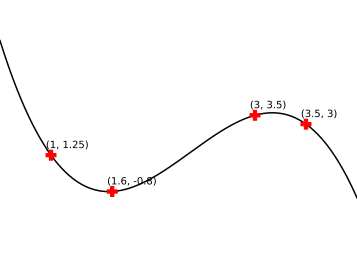
\includegraphics[width=.5\textwidth]{pictures/newton_polynomial}
        \vspace{-1em}
    \end{figure}

\end{tcolorbox}

Let us now derive Simpson's rule. We define three equally spaced points (with step size $h$) and denote them as $x_0$, $x_1=x_0+h$ and $x_2=x_0+2h$ and their corresponding function values by $f_0$, $f_1$ and $f_2$, respectively. To form the Newton polynomial, we first write the points in the form of equation \ref{eq:newton_pol}:
\begin{equation}
    \begin{matrix}
        x_0 & f_0 \\
            & & \frac{f_1-f_0}{h} \\
        x_1 & f_1 & & \frac{f_0 + f_2-2f_1}{2h^2} \\
            & & \frac{f_2-f_1}{h} \\
        x_2 & f_2 \\
    \end{matrix} \,.\nonumber
\end{equation}
The interpolating polynomial then becomes
\begin{equation}
    p(x) = f_0 + \frac{f_1-f_0}{h} (x-x_0) + \frac{f_0 + f_2-2f_1}{2h^2} (x-x_0)(x-x_1) \,.\nonumber
\end{equation}
Integrating from $x_0$ to $x_2$ (keeping in mind that $x_1-x_0 = h$ and $x_2-x_0 = 2h$) now gives us Simpson's rule:
\begin{align}
    \int_{x_0}^{x_2} p(x) \mathrm dx &= \left[f_0 x + \frac{f_1-f_0}{2h} (x-x_0)^2 + \frac{f_0 + f_2-2f_1}{2h^2} \left(\frac{x^3}{3}-(x_0+x_1)\frac{x^2}{2} + x_0 x_1 x\right)\right]_{x_0}^{x_2} \nonumber \\
                                     &= 2hf_0 + 2h(f_1-f_0) + \frac{f_0 + f_2-2f_1}{2h^2} \left(\frac{x_2^3-x_0^3}{3}-(x_0+x_1)\frac{x_2^2-x_0^2}{2} + 2h x_0 x_1 \right) \nonumber \\
                                     &= 2hf_1 + \frac{f_0 + f_2-2f_1}{2h^2} \left(\frac{8h^3}{3}+2x_0^2h+4x_0h^2-(2h^2+2hx_0)(2x_0+h) + 2h x_0 (x_0+h) \right) \nonumber \\
                                     &= 2hf_1 + \frac{f_0 + f_2-2f_1}{2h^2} \left(\frac{2h^3}{3}+4x_0^2h+2x_0h^2-2hx_0(2x_0+h)  \right) \nonumber \\
                                     &= 2hf_1 + \frac{f_0 + f_2-2f_1}{2h^2} \frac{2h^3}{3} \nonumber \\
                                     &= 2hf_1 + \frac{h}{3}(f_0 + f_2-2f_1) \nonumber \\
                                     &= \frac{h}{3}(f_0 + 4f_1 + f_2) \,.\nonumber
\end{align}
In Subsection \ref{newton_cotes_integrals} we explain how one can use this result to approximate integrals, together these section form the basis for the combined interpolation method in Chapter \ref{chap4}.

\subsection{Cotesian numbers}
\label{sec:cotesian}
Instead of interpolating $3$ points by a parabola, we can also interpolate $n+1$ points by an $n$th-order polynomial (we note that the order can be lower than $n$), by doing this, we obtain the Cotesian numbers used in Newton-Cotes equations.
Higher order equations can be more accurate in approximating integrals than Simpson's rule.

We will denote the Cotesian numbers as $c_0$, $c_1$, $\dots$, $c_n$, which are defined such that after defining points $x_0$, $x_1$, \dots, $x_n$ and function values $f_0$, $f_1$, $\dots$, $f_n$ the integral over the interpolated polynomial can be approximated by $h(c_0f_0+c_1f_1+\cdots+c_nf_n)$, where $h$ is the distance between two points $x_i$ and $x_{i+1}$.

To calculate the Cotesian numbers, we can solve the following system of equations (the proof of this statement is in Appendix \ref{app:proofs} as the proof of Theorem \ref{theorem:mat}):
\begin{equation}
    \begin{bmatrix}
        1&0&0&\cdots&0 \\
        1&1&1&\cdots&1 \\
        1&2&2^2&\cdots&2^n \\
        \vdots&\vdots & \vdots & \ddots & \vdots\\
        1&n&n^2&\cdots&n^n
    \end{bmatrix}^\top
    \begin{bmatrix}
        c_0\\
        c_1\\
        c_2\\
        \vdots \\
        c_n
    \end{bmatrix}
    =
    \begin{bmatrix}
        n/1 \\
        n^2/2 \\
        n^3/3 \\
        \vdots \\
        n^{n+1}/(n+1)
    \end{bmatrix} \,,\nonumber
\end{equation}
where the matrix on the left-hand side is the Vandermonde matrix.
Since the inverse of the Vandermonde matrix exists in closed form (see Lemma \ref{lemma:invertible} in Appendix \ref{app:proofs}), the matrix can be brought to the other side \cite{vandermonde_inv}.
After denoting the signed Stirling numbers of the first kind as $s(n, k)$ and doing just that we get a non-recursive formula for the coefficients $c_i$ for $0 \leq i \leq n$ (Theorem \ref{theorem:calc} in Appendix \ref{app:proofs}):
\begin{equation}
    c_i = \frac{1}{(n-1)!} \binom{n}{i} \sum_{j=0}^{n} \sum_{m=0}^{n-j} i^m n^{j} \frac{(-1)^{i+n} s(n+1, j+m+1) }{j+1} \,. \nonumber
\end{equation}
% \begin{equation}
%     c_i =
%     \begin{dcases}
%         \frac{1}{(n-1)!}\sum\limits_{k=1}^{n} \frac{n^k s(n, k)}{k+1} & i = 0 \text{ or } i=n\\
%         \frac{1}{(n-1)!}\binom{n}{i}\sum\limits_{j=1}^{i} \sum\limits_{k=1}^{n-i} n^{j+k} \frac{s(i, j)s(n-i, k)}{(k+1)\binom{j+k+1}{k+1}} & \text{otherwise}
%     \end{dcases}\nonumber
% \end{equation}
For simplicity, one can also look these numbers up, since they constitute a sequence in the OEIS (the On-Line Encyclopedia of Integer Sequences, \url{http://oeis.org/}). In terms of these sequences\footnote{For the corresponding sequences we refer the reader to OEIS Foundation Inc. (2022), Denominators of Cotesian numbers, Entry \href{http://oeis.org/A002176}{A002176} and Numerators of Cotesian numbers, Entry \href{http://oeis.org/A100642}{A100642} in The On-Line Encyclopedia of Integer Sequences, \url{http://oeis.org/A002176} and \url{http://oeis.org/A100642}.} we can write the Cotesian numbers as:
\begin{equation}
    \frac{nh}{\textrm{A002176}(n)} \left[\sum_{i=0}^n \textrm{A100642}\left(\frac{n(n+1)}{2} + i\right)f_i \right] \,. \nonumber
\end{equation}
The Cotesian numbers then determine the Newton-Cotes equations that can be used for approximating integrals:
\begin{gather}
    \frac{h}{2}(f_0 + f_1) \nonumber \\
    \frac{h}{3}(f_0+4f_1+f_2) \nonumber \\
    \frac{3h}{8}(f_0 + 3f_1 + 3f_2 + f_3) \nonumber \\
    \frac{2h}{45}(7f_0 + 32f_1 + 12f_2 + 32f_3 + 7f_4) \nonumber \\
    \frac{5h}{288}(19f_0 + 75f_1 + 50f_2 + 50f_3 + 75f_4 + 19f_5) \nonumber \\
    \frac{h}{140}(41f_0 + 216f_1 + 27f_2 + 272f_3 + 27f_4 + 216f_5 + 41f_6) \nonumber \\
    \frac{7h}{17280}(751f_0 + 3577f_1 + 1323f_2 + 2989f_3 + 2989f_4 + 1323f_5 + 3577f_6 + 751f_7) \,. \nonumber \\
    \udots \hspace{5em} \vdots \hspace{5em} \vdots \hspace{5em} \vdots \hspace{5em} \ddots \label{eq:newton_cotes}
    % & \frac{4h}{14175}(989f_0 + 5888f_1 - 928f_2 + 10496f_3 - 4540f_4 + 10496f_5 - 928f_6 + 5888f_7 + 989f_8) \nonumber \\
    % & \frac{9h}{89600}(2857f_0 + 15741f_1 + 1080f_2 + 19344f_3 + 5778f_4 + 5778f_5 + 19344f_6 + 1080f_7 + 15741f_8 + 2857f_9) \nonumber \\
    % & \frac{5h}{299376}(16067f_0 + 106300f_1 - 48525f_2 + 272400f_3 - 260550f_4 + 427368f_5 - 260550f_6 + 272400f_7 - 48525f_8 + 106300f_9 + 16067f_{10}) \nonumber \\
    % & \frac{11h}{87091200}(2171465f_0 + 13486539f_1 - 3237113f_2 + 25226685f_3 - 9595542f_4 + 15493566f_5 + 15493566f_6 - 9595542f_7 + 25226685f_8 - 3237113f_9 + 13486539f_{10} + 2171465f_{11}) \nonumber \\
    % & \frac{h}{5255250}(1364651f_0 + 9903168f_1 - 7587864f_2 + 35725120f_3 - 51491295f_4 + 87516288f_5 - 87797136f_6 + 87516288f_7 - 51491295f_8 + 35725120f_9 - 7587864f_{10} + 9903168f_{11} + 1364651f_{12}) \nonumber \\
    % & \frac{13h}{402361344000}(8181904909f_0 + 56280729661f_1 - 31268252574f_2 + 156074417954f_3 - 151659573325f_4 + 206683437987f_5 - 43111992612f_6 - 43111992612f_7 + 206683437987f_8 - 151659573325f_9 + 156074417954f_{10} - 31268252574f_{11} + 56280729661f_{12} + 8181904909f_{13}) \nonumber \\
    % & \frac{7h}{2501928000}(90241897(f_0+f_{14}) + 710986864(f_1+f_{13}) - 770720657(f_2+f_{12}) + 3501442784(f_3+f_{11}) - 6625093363(f_4+f_{10}) + 12630121616(f_5+f_9) - 16802270373(f_6+f_8) + 19534438464f_7) \nonumber
\end{gather}
More information on this subject is only referenced \cite{cotesian1, cotesian2}.


\subsection{From Newton-Cotes equations to integrals}
\label{newton_cotes_integrals}
We now give the method for extending the Newton-Cotes equations to evaluate integrals.
Let us integrate over the interval $[x_L, x_R]$.
Partitioning this interval into the subintervals $[x_0, x_1]$, \dots, $[x_i, x_{i+1}]$, \dots $[x_{\ell-1}, x_{\ell}]$ with $x_0 = x_L$ and $x_\ell = x_R$, whilst noting that the subintervals do not have to be equidistant, allows us to approximate the integral over each subinterval by applying an $n$th-order Newton-Cotes equation (note that the order is allowed change for different subintervals) to that subinterval by defining the function values to be $f_0=f(x_i)$, $f_1 = f(x_i+\frac{x_{i+1}-x_i}{n})$, \dots, $f_k = f(x_i + k\frac{x_{i+1}-x_i}{n})$ \dots, $f_n = f(x_{i+1})$.

If we partition the original interval $[x_L, x_R]$ into equidistant subintervals and always apply Simpson's rule to the subinterval, we get the same effect as the following equation (where we evaluated the function at points $x_0, \dots, x_n$ with $x_0=x_L$ and $x_n = x_R$)
\begin{equation}
    \int_{x_L}^{x_R} f(x) \mathrm d x \approx \frac{h}{3}(f_0 + 4 f_1 + 2 f_2 + 4f_3 + \dots + 2 f_{n-2} + 4 f_{n-1} + f_n) \,.\nonumber
\end{equation}
This way, between every $3$ points $f_{2i}, f_{2i+1}, f_{2i+2}$ we interpolate the points by a parabola, integrate the parabola from $x_{2i}$ to $x_{2i+2}$, and we add up the results to approximate our integral.

Provided that we can split up the subintervals into the number of equidistant parts needed for the Newton-Cotes equations, we can also use vector notation to approximate the integral, for the above example this works out to be
\begin{equation}
    \int_{x_L}^{x_R} f(x) \mathrm d x \approx \mathbf c\mathbf f^\top \,,\nonumber
\end{equation}
with
\begin{equation}
    \mathbf c = \frac{h}{3}\begin{bmatrix}1&4&2&4&\dots&2&4&1\end{bmatrix}\quad \textrm{and} \quad
    \mathbf f = \begin{bmatrix}f_0&f_1&\dots&f_n\end{bmatrix} \,. \label{eq:vectors}
\end{equation}


\section{Examples}
\label{examples}
In this section we give numerical examples of approximating integrals using the methods described in previous sections of this chapter.
The examples provide an overview of the described methods and give an idea of what their accuracy is and where we can find room for improvement.
This section can also function as a tool to check the implementation of other researchers wanting to implement these methods themselves (note that the code to our implementation can be found in Appendix \ref{app:code}).

We start by interpolating functions using various types of polynomials.
The first type is $N_1$, the 1st-order Newton-Cotes equation known as the trapezoidal rule (this uses linear interpolation) for which the integral can be found at the top in equation \ref{eq:newton_cotes}.
This type is currently most commonly used for evaluating the Rayleigh integral and is therefore added as a benchmark.
The second type is $N_2$, the 2nd-order Newton-Cotes equation known as Simpson's rule.
The third type is $S_3$, a cubic spline interpolation.
Results of the interpolation can be seen in Figure \ref{fig:res_1}.
\begin{figure}[H]
    \vspace{-.5em}
    \begin{tabular}{rl}
        \subcaptionbox{\centering Interpolation of $h_1(x)$.}{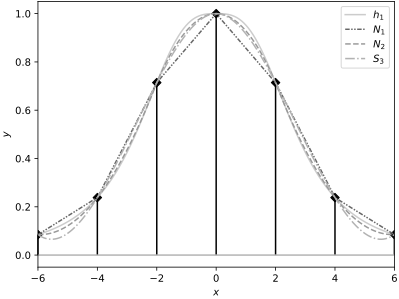
\includegraphics[width=.46\textwidth]{pictures/interpolate_func1}} &
        \subcaptionbox{\centering Interpolation of $h_2(x)$.\label{fig:res_1b}}{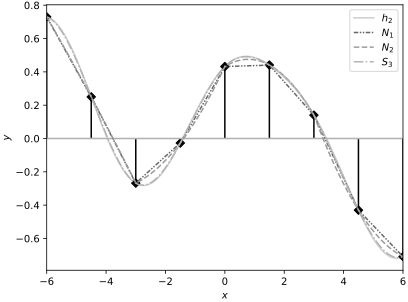
\includegraphics[width=.47\textwidth]{pictures/interpolate_func2}} \\
        \subcaptionbox{\centering Difference between interpolated functions and $h_1(x)$.\label{fig:diff_c}}{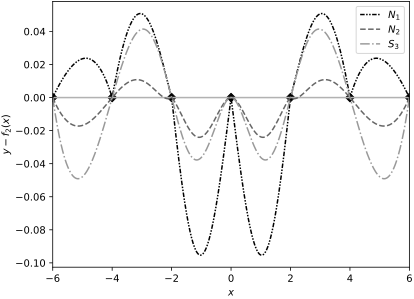
\includegraphics[width=.47\textwidth]{pictures/difference_func1}} &
        \subcaptionbox{\centering Difference between interpolated functions and $h_2(x)$.}{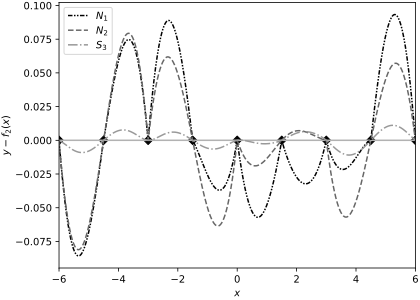
\includegraphics[width=.47\textwidth]{pictures/difference_func2}}
    \end{tabular}
    \vspace{-.2em}
    \caption{Interpolation of $h_1(x) = 1/(1+|x|^3/20)$ and $h_2(x) = \cos(\sqrt{(x-1)^2/4+1}) \cdot \sin(\sqrt{(x-2)^2/4+1})$ using $7$ and $9$ sample points of the function, respectively.}
    \label{fig:res_1}
    \vspace{-.8em}
\end{figure}
The integrals over the various interpolation types are listed in Table \ref{tab:res_1}, where a few are calculated explicitly later on in this section.
To illustrate how polynomials of higher order behave we have added a fourth type: $N_6$ (and the type $N_{1-6-1}$, which is the same as $N_6$ enclosed by two $N_1$'s to account for the number of sample points), being the 6th-order Newton-Cotes equation.

From Table \ref{tab:res_1} and Figure \ref{fig:res_1} we can see that $N_1$ got lucky with good approximation for the integral over function $h_1(x)$, since although $N_1(x) - h_1(x)$ (Figure \ref{fig:diff_c}) has the greatest deflections the resulting integral is very close to the actual integral because the average deflection is coincidentally close to zero.
However, with the other function ($h_2(x)$) the interpolation is less lucky, as other methods now give significantly better approximation to the integral.
\begin{table}[H]
    \vspace{-0.5em}
    \centering
    \begin{tabular}{p{.47\textwidth}p{.47\textwidth}}
        \begin{tabular}{cccc}
            Func. & Integral & Abs. diff. & Rel. diff. \\
            \hline
            $h_1(x)$ & $6.02845$ & - & - \\
            $N_1$    & $5.97902$ & $0.04943$ & $0.820\%$ \\
            $N_2$    & $5.95426$ & $0.07419$ & $1.23\%$ \\
            $N_6$    & $6.00540$ & $0.02305$ & $0.382\%$ \\
            $S_3$    & $5.92113$ & $0.10732$ & $1.78\%$
        \end{tabular} &
        \begin{tabular}{cccc}
            Func. & Integral & Abs. diff. & Rel. diff. \\
            \hline
            $h_2(x)$ & $0.79728$ & - & - \\
            $N_1$    & $0.82342$ & $0.02615$ & $3.28\%$ \\
            $N_2$    & $0.78280$ & $0.01448$ & $1.82\%$ \\
            $N_{1-6-1}$ & $0.88535$ & $0.08807$ & $11.0\%$ \\
            $S_3$    & $0.79930$ & $0.00203$ & $0.254\%$
        \end{tabular}
    \end{tabular}
    \vspace{-.2em}
    \caption{Various interpolations of function $h_1(x)$ on the left side and $h_2(x)$ on the right side together with the absolute difference and the relative difference between the integral and the correct integral.}
    \label{tab:res_1}
    \vspace{-0.5em}
    \centering
\end{table}
The large error in the approximation using $N_{1-6-1}$ is due to the boundaries of $N_6$.
These have great deflections causing an inaccurate result.
A method to remove the error would be to derive the coefficients using the integral, but instead of integrating over the full interval we can integrate over a subsection of it.
For the 6th-order Newton-Cotes equation we can take the integral from $x_1$ to $x_5$, resulting in the following formula (the original one can be found in equation \ref{eq:newton_cotes}):
\begin{equation}
   \frac{2h}{945}(-4f_0 + 171f_1 + 612f_2 + 332f_3 + 612f_4 + 171f_5 - 4f_6) \,. \label{eq:6star}
\end{equation}
We can then evaluate the integral of $h_2(x)$ again with an $N_{2-6^*-2}$ interpolation (we need to pad with two $N_2$'s since the new $N_{6^*}$ is integrated over fewer points), also we note that in the above formula the endpoints ($f_0$ and $f_6$) are weighted less since they do not directly contribute to the integral, only indirectly by interpolation.
The approximation for the integral becomes 0.77928, with an absolute difference of 0.01800 and a relative difference of 2.26\%.
This is a huge improvement compared to the relative error of 11.0\% from using $N_{1-6-1}$.
However, we do not investigate these methods further as the method still performes worse than $N_2$ and $S_3$ (this is instead left to future research in Section \ref{discussion}) and only polynomials up to the 2nd-order are used hereafter.

The best methods from above are therefore $N_2$ and $S_3$, however, since this is still combined interpolation (Section \ref{comb_interpol}) the integrals can also be approximated using separate interpolation (Section \ref{sep_interpol}).

We compare the combined interpolation using $S_3$ (thus we interpolate $f(x)\cdot g(x)$ by a cubic spline) and the separate interpolation using $S_3$ (thus we interpolate $f(x)$ and $g(x)$ separately where we interpolate $f(x)$ by a cubic spline and $g(x)$ to a high degree since it is known and combine the results by the method described in Section \ref{sep_interpol}).
The difference between the functions and their interpolations can be seen in Figure \ref{fig:res_2}, where we note that $h_2(x) = f_2(x)\cdot g_2(x)$ but that $h_1(x) \neq f_1(x)\cdot g_1(x)$ due to the function that was chosen.
The corresponding differences are listed in Table \ref{tab:res_2}, and the calculation of $S_3$ -- S can be found at the end of this section.
\begin{table}[H]
    \centering
    \begin{tabular}{p{.4\textwidth}p{.4\textwidth}}
        % \subcaptionbox{hihi}{\begin{tabular}{r} hi \\ hi \end{tabular}}
        % \subcaptionbox{hihi}{\begin{tabular}{r} hi \\ hi \end{tabular}}
        \subcaptionbox{The integral is approximately $4.60931999$.}{
        \begin{tabular}{ccc}
            Method &  Abs. diff. & Rel. diff. \\
            \hline
            $S_3$ -- C &  $0.001156$ & $0.0251\%$ \\
            $S_3$ -- S &  $0.0001215$ & $0.00264\%$ \\
        \end{tabular}} &
        \subcaptionbox{The integral is approximately $0.79727674$.}{
        \begin{tabular}{ccc}
            Method &  Abs. diff. & Rel. diff. \\
            \hline
            $S_3$ -- C &  $0.00202819$ & $0.254\%$ \\
            $S_3$ -- S &  $0.00174655$ & $0.219\%$ \\
        \end{tabular}}
    \end{tabular}
    \vspace{-.2em}
    \caption{The absolute difference and the relative difference between the integral and the correct integral using combined and separate interpolation techniques. For the functions we used $f_1(x)\cdot g_1(x)$ on the left-hand side and $f_2(x)\cdot g_2(x)$ on the right-hand side, see the caption of Figure \ref{fig:res_2} for the corresponding functions.}
    \label{tab:res_2}
    \vspace{-.5em}
\end{table}

The separate interpolation method is better than the combined method as can be seen in Figure \ref{fig:res_2} and Table \ref{tab:res_2}.
However, the large difference from the second function on the left side of the interval was not compensated, resulting in a high overall difference that does not do the method justice.
\begin{figure}[H]
    % \vspace{-10pt}
    \begin{tabular}{rl}
        \subcaptionbox{\centering Difference between interpolation and $f_1(x)\cdot g_1(x)$.}{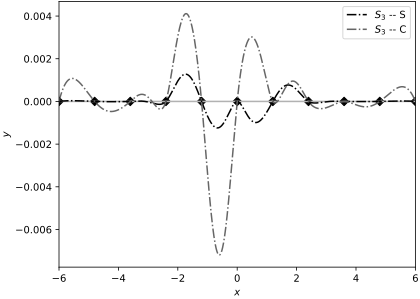
\includegraphics[width=.46\textwidth]{pictures/interpolate_spline_func1}} &
        \subcaptionbox{\centering Difference between interpolation and $f_2(x)\cdot g_2(x)$.}{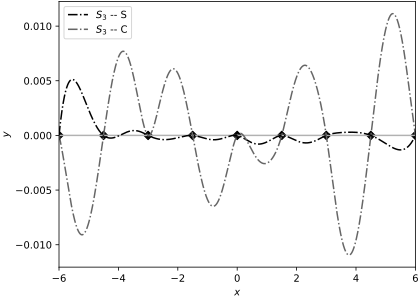
\includegraphics[width=.47\textwidth]{pictures/interpolate_spline_func2}}
    \end{tabular}
    \vspace{-.2em}
    \caption{In these figures $f_1(x) = 1/(1+x^2/10)$, $g_1(x) = 1/(1+(x+1)^2/10)$ and $f_2(x) = \cos(\sqrt{(x-1)^2/4+1})$, $g_2(x) = \sin(\sqrt{(x-2)^2/4+1})$. Interpolation was done on 11 and 9 samples points, respectively, by means of a separate interpolation method denoted by $S_3$ -- S and a combined interpolation method denoted by $S_3$ -- C.}
    \label{fig:res_2}
\end{figure}

\subsubsection{Calculating the integrals using the Newton-Cotes equations by interpolating $h_2(x)$}
We provide example calculations of using various Newton-Cotes equations to approximate the integral over $h_2(x)$, the general methods are presented in Section \ref{comb_interpol}.

The function values of $h_2(x)$ at the 9 samples points from Figure \ref{fig:res_1b} written in vector notation are:
\begin{equation}
    \scalemath{0.99}{
    \mathbf f =
    \begin{bmatrix}
        0.73018 & 0.24998 & -0.26794 & -0.02706 & 0.4321 & 0.44099 & 0.14023 & -0.43006 & -0.70876
    \end{bmatrix} \,.} \nonumber
\end{equation}
The value for $h$ can be calculated by dividing the total width of the interval by the total number of subintervals (which is one less than the number of sample points):
\begin{equation}
    h = \frac{12}{9-1} = \frac{3}{2} \,.\nonumber
\end{equation}
Now, for all different interpolating polynomials $N_1$, $N_2$, $N_{1-6-1}$, and $N_{2-6^*-2}$ we determine the corresponding vector from equation \ref{eq:vectors} (note that the coefficients can be found in equations \ref{eq:newton_cotes} and \ref{eq:6star}):
\begin{equation}
    \mathbf c_1 = \frac{3}{4}
    \begin{bmatrix}
        1 & 2 & 2 & 2 & 2 & 2 & 2 & 2 & 1
    \end{bmatrix} \,, \quad
    \mathbf c_2 = \frac{1}{2}
    \begin{bmatrix}
        1 & 4 & 2 & 4 & 2 & 4 & 2 & 4 & 1
    \end{bmatrix} \,,\nonumber
\end{equation}
\begin{equation}
    \mathbf c_{1-6-1} = \begin{bmatrix}
        \frac{3}{4} & \frac{3}{4} + \frac{3\cdot 41}{280} & \frac{3\cdot 216}{280} & \frac{3\cdot 27}{280} & \frac{3\cdot 272}{280} & \frac{3\cdot 27}{280} & \frac{3\cdot 216}{280} & \frac{3\cdot 41}{280} + \frac{3}{4} & \frac{3}{4}
    \end{bmatrix} \,,\nonumber
\end{equation}
\begin{equation}
    \mathbf c_{2-6^*-2} = \begin{bmatrix}
        \frac{1}{2} & 2 - \frac{3\cdot 4}{945} & \frac{1}{2}+\frac{3\cdot 171}{945} & \frac{3\cdot 612}{945} & \frac{3\cdot 332}{945} & \frac{3\cdot 612}{945} & \frac{3\cdot 171}{945}+\frac{1}{2} & -\frac{3\cdot 4}{945} + 2 & \frac{1}{2}
    \end{bmatrix} \,.\nonumber
\end{equation}
Now, we can finally approximate the integral by determining the integral over $N_1$, $N_2$, $N_{1-6-1}$, and $N_{2-6^*-2}$, this can thus be done without ever having to interpolate the function:
\begin{equation}
    \mathbf c_1 \mathbf f^\top \approx 0.823425 \,, \quad
    \mathbf c_2 \mathbf f^\top \approx 0.782800 \,, \quad
    \mathbf c_{1-6-1} \mathbf f^\top \approx 0.885348 \,, \quad
    \mathbf c_{2-6^*-2} \mathbf f^\top \approx 0.779280 \,. \nonumber
\end{equation}
Verifying the results in Table \ref{tab:res_1} and below.

\subsubsection{Calculating the integral over $f_2(x) \cdot g_2(x)$ using separate spline interpolation}
To replicate the results from Table \ref{tab:res_2} we first write $f_2(x)$ and $g_2(x)$ without subscripts, i.e. $f(x)$ and $g(x)$, to avoid confusion later on.
In this example we have used $n_f=3$ and $n_g = 5$.

To avoid rounding errors we modify the method in Section \ref{sep_interpol}, avoiding any high powers of $x_i$ when calculating the various values of $d_{ij}$.
The modification of the method is to shift all the subintervals $[x_i, x_{i+1}]$ to $[x_4, x_5] = [0, \frac{3}{2}]$ and carry out the interpolation for all the subintervals on this new domain.
Using this method we only need to calculate powers of $x_4=0$ and $x_5=\frac{3}{2}$ instead of powers of $x_i$ and $x_{i+1}$, this speeds up the process and avoids multiplying by large numbers resulting in less rounding errors in our answer.
For the shifted interpolation the coefficients of the interpolating polynomial of $f_3(x)$ (i.e. $\mathbf b_{3j}$) are now the coefficients after interpolating $f_3(x-\frac{3}{2})$ on the interval $[0, \frac{3}{2}]$.
Similarly, the coefficients for $\mathbf b_{1j}$ are the coefficients from interpolating $f_1(x-3\cdot \frac{3}{2})$ on the interval $[0, \frac{3}{2}]$.
To obtain the correct answer using these shifted interpolation coefficients we need to make a second adjustment to our method.
This is for calculating the values of $d_{ij}$ (equation \ref{eq:calc_dij}).
We need to use the values $x_4$ and $x_5$ repeatedly instead of $x_{i}$ and $x_{i+1}$, respectively.
Since $x_4=0$ this results in calculating and storing the values of $x_{5}^{j+k+1}/(j+k+1)$ for all values of $j+k$ before calculating (and storing if we have multiple sensors) the values of
\begin{equation}
    d_{ij} = \sum_{k=0}^{n_g} c_{ik} \frac{x_{5}^{j+k+1}}{j+k+1} \,. \nonumber
\end{equation}
All things considered, these modifications improve the accuracy of our results as they avoid rounding errors.

The function $f_3(x-\frac{3}{2})$ interpolated on $[x_4, x_5] = [0, \frac{3}{2}]$ is given as:
\begin{equation}
    f_3\left(x-\frac{3}{2}\right) \approx -0.02998 + 0.39005 x -0.03051 x^2 -0.014518 x^3 \,, \nonumber
\end{equation}
resulting in row $3$ of matrix $B$,
\begin{equation}
    \mathbf b_{3j} = \begin{bmatrix}-0.02998 & 0.39005 & -0.03051 & -0.014518 \end{bmatrix} \,. \nonumber \\
\end{equation}
Continuing this process to calculate all elements of $B$ and $C$ we can calculate the elements of $D$ and use equation \ref{eq:final_int} to approximate the integral.
In Appendix \ref{app:matrices} we listed all values of the matrices.
We note that the method seems like a lot of work, but after we initialize it we can easily calculate the sum in equation \ref{eq:final_int} again with a shift to approximate the integral for a different sensor.

Taking everything into account, using this method we get a value of $0.79902$ for the evaluation of the integral, which corresponds to an absolute difference of $0.00175$ and a relative difference of $0.219\%$.
Without the method of shifting the intervals we would have obtained the value $0.79958$ with a relative difference of $0.289\%$, due to rounding errors resulting from multiplying by a factor of $(x_{i+1}^{j+k+1} - x_i^{j+k+1})/(j+k+1)$.

The obtained value can be improved upon (by a tiny fraction) by increasing the order of the spline (or polynomial) used to interpolate $g(x)$, i.e. increasing $n_g$.

\chapter{Adapting numerical integration methods for the Rayleigh integral}
\label{chap4}
In this chapter we adapt the numerical methods from Chapter \ref{chap3} to better fit the Rayleigh integral (equation \ref{eq:rayleigh}).
The methods we develop will be compared in Chapter \ref{chap5}, the results of this thesis.

The first section will generalize both methods derived in the previous chapter (Section \ref{sep_interpol} for separate interpolation and Section \ref{comb_interpol} for combined interpolation) to complex, double integrals.
In the next section we present a variation to the combined interpolation method (Section \ref{comb_interpol}), in specific Simpson's rule, to evaluate integrals on non-equidistant intervals (single integrals) and semi-equidistant grids (double integrals), weakening the assumption made in Chapter \ref{chap3} of an equidistant grid.
In the last section we summarize all the derived methods and their qualities for the next chapter, where we present the results of evaluating an artificial Rayleigh integral using those methods.

\section{From single to double integrals}
The Rayleigh integral is not a real-valued, single integral. It is a complex valued, double integral.
Therefore, in this section, we present methods that extend the algorithms from Sections \ref{sep_interpol} and \ref{comb_interpol} to complex-valued, double integrals.
Using these new methods we can approximate the Rayleigh integral in three dimensions, giving us the ability to propagate a wavefield from one layer of soil to the next.

\subsection{Separate interpolation}
\label{sep_interpol_3d}
This argument is very similar to the one in Section \ref{sep_interpol}.
However, since this is a key element of the implementation of this thesis we will write it out.
This extension does not include the complex-valued integral.
We note that to calculate it one could use the method described below for the real-real values of $f$ and $g$, the imaginary-real, the real-imaginary and the imaginary-imaginary (as a consequence the initialization of the algorithm only takes twice as long whereas the evaluation takes 4 times as long), after combining the results one finds the integral.

The interval $[x_L,x_R]\times [y_L, y_R]$ is partitioned into $\ell_x \cdot \ell_y$ equally large subintervals
\begin{equation}
    \begin{matrix}
    % \begin{array}{ccrc}
        [x_0, x_1]\times[y_0, y_1] & [x_0, x_1]\times[y_1, y_2] & \cdots & [x_0, x_1]\times[y_{\ell_y-1}, y_{\ell_y}] \\
        [x_1, x_2]\times[y_0, y_1] & [x_1, x_2]\times[y_1, y_2] & \cdots & [x_1, x_2]\times[y_{\ell_y-1}, y_{\ell_y}] \\
        \vdots & \vdots & \ddots & \vdots \\
        [x_{\ell_x-1}, x_{\ell_x}]\times[y_0, y_1] & [x_{\ell_x-1}, x_{\ell_x}]\times[y_1, y_2] & \cdots &  [x_{\ell_x-1}, x_{\ell_x}]\times [y_{\ell_y-1}, y_{\ell_y}]
    % \end{array}
    \end{matrix}\,,
    \nonumber
\end{equation}
that is, $x_1 - x_0 =\cdots = x_{\ell_x} - x_{\ell_x-1}$, $x_L = x_0$, and $x_R = x_{\ell_x}$ and $y_1 - y_0 = \cdots = y_{\ell_y} - y_{\ell_y-1}$, $y_L = y_0$, and $y_R = y_{\ell_y}$.

For each interval $[x_{i_x}, x_{i_x+1}]\times[y_{i_y}, y_{i_y+1}]$ with $0 \leq i_x \leq \ell_x -1$ and $0 \leq i_y \leq \ell_y -1$ both functions are interpolated by polynomials \cite{2dpol_inter}:
\begin{equation}
    f_{i_x, i_y}(x, y) = \sum_{j_x=0}^{n_f}\sum_{j_y=0}^{m_f} b_{i_xi_yj_xj_y} x^{j_x}y^{j_y} \,,  \quad
    g_{i_x, i_y}(x, y) = \sum_{k_x=0}^{n_g}\sum_{k_y=0}^{m_g} c_{i_xi_yk_xk_y} x^{k_x}y^{k_y} \,. \nonumber
\end{equation}
Using the fact that the intervals are equidistant the interpolation can be achieved with a time complexity of $\mathcal O(n_f^2m_f^2 \ell_x \ell_y + n_g^2m_g^2 \ell_x \ell_y)$, we also need $\mathcal O(n_fm_f\ell_x\ell_y + n_gm_g\ell_x\ell_y)$ space.

We assume the prediction points (the points corresponding to different values of $a_x$, $a_y$) are spaced in an equidistant grid (this is often the case).
We write $a_x = m_x (x_1 - x_0)$ and $a_y = m_y(y_1-y_0)$ with $m_x\in \mathbb N$, $m_y \in \mathbb N$, $0\leq m_x \leq s_x$ and $0\leq m_y \leq s_y$, where $s_x$ denotes the number of prediction points in the $x$-direction and $s_y$ those in the $y$-direction, such that the integral becomes (we make the same assumption that $f(x,y)=g(x,y)=0$ for $(x,y) \notin [x_L, x_R]\times[y_L,y_R]$):
\begin{align}
    \int_{y_L}^{y_R} \int_{x_L}^{x_R} &f(x', y') g(x'+a_x, y'+a_y) \mathrm d x'\mathrm d y' \nonumber \\
    &= \int_{y_L-a_y}^{y_R-a_y} \int_{x_L-a_x}^{x_R-a_x} f(x-a_x, y-a_y) g(x, y) \mathrm d x\mathrm d y \nonumber \\
                                                &\approx \sum_{i_x=0}^{\ell_x-m_x}\sum_{i_y=0}^{\ell_y-m_y} \int_{y_{i_y}}^{y_{i_y+1}} \int_{x_{i_x}}^{x_{i_x+1}} f_{i_x, i_y}(x-a_x, y-a_y) g_{i_x, i_y}(x, y) \mathrm d x \mathrm d y \nonumber \\
                                                &= \sum_{i_x=0}^{\ell_x-m_x}\sum_{i_y=0}^{\ell_y-m_y} \int_{y_{i_y}}^{y_{i_y+1}} \int_{x_{i_x}}^{x_{i_x+1}} f_{i_x+m_x, i_y+m_y}(x) g_{i_x, i_y}(x) \mathrm d x \nonumber \\
                                                &= \sum_{i_x=0}^{\ell_x-m_x}\sum_{i_y=0}^{\ell_y-m_y} \int_{y_{i_y}}^{y_{i_y+1}} \int_{x_{i_x}}^{x_{i_y+1}} \sum_{j_x=0}^{n_f}\sum_{j_y=0}^{m_f}\sum_{k_x=0}^{n_g}\sum_{k_y=0}^{m_g} b_{i_x+m_x,i_y+m_y,j_x,j_y} c_{i_xi_yk_xk_y} x^{j_x+k_x}y^{j_y+k_y} \mathrm d x \mathrm d y \nonumber \\
                                                &= \sum_{i_x=0}^{\ell_x-m_x}\sum_{i_y=0}^{\ell_y-m_y} \sum_{j_x=0}^{n_f}\sum_{j_y=0}^{m_f}\sum_{k_x=0}^{n_g}\sum_{k_y=0}^{m_g} b_{i_x+m_x,i_y+m_y,j_x,j_y} c_{i_xi_yk_xk_y}  \int_{y_{i_y}}^{y_{i_y+1}} \int_{x_{i_x}}^{x_{i_x+1}}  x^{j_x+k_x}y^{j_y+k_y} \mathrm d x \mathrm d y \nonumber \\
                                                &= \sum_{i_x=0}^{\ell_x-m_x}\sum_{i_y=0}^{\ell_y-m_y} \sum_{j_x=0}^{n_f}\sum_{j_y=0}^{m_f} b_{i_x+m_x,i_y+m_y,j_x,j_y} \sum_{k_x=0}^{n_g}\sum_{k_y=0}^{m_g} c_{i_xi_yk_xk_y} \frac{x_{i_x+1}^{j_x+k_x+1} - x_{i_x}^{j_x+k_x+1}}{j_x+k_x+1}  \frac{y_{i_y+1}^{j_y+k_y+1} - y_{i_y}^{j_y+k_y+1}}{j_y+k_y+1} \,.\nonumber
\end{align}
Storing the values of
\begin{equation}
    d_{i_xi_yj_xj_y} = \sum_{k_x=0}^{n_g}\sum_{k_y=0}^{m_g} c_{i_xi_yk_xk_y} \frac{x_{i_x+1}^{j_x+k_x+1} - x_{i_x}^{j_x+k_x+1}}{j_x+k_x+1}  \frac{y_{i_y+1}^{j_y+k_y+1} - y_{i_y}^{j_y+k_y+1}}{j_y+k_y+1} \,, \nonumber
\end{equation}
for all $i_x,i_y$ and $j_x,j_y$, then allows us to rewrite the equation, giving:
\begin{equation}
    \int_{y_L}^{y_R}\int_{x_L}^{x_R} f(x,y) g(x+a_x,y+a_y) \mathrm d x \mathrm dy \approx \sum_{i_x=0}^{\ell_x-m_x}\sum_{i_y=0}^{\ell_y-m_y} \sum_{j_x=0}^{n_f}\sum_{j_y=0}^{m_f} b_{i_x+m_x,i_y+m_y,j_x,j_y} d_{i_xi_yj_xj_y} \,.\nonumber
\end{equation}
% The process of storing the values of $d_{i_x,i_y,j_x,j_y}$ has a space and time complexity of $\mathcal O(n_fm_f\ell_x + n_gm_g\ell_y)$. After which computing the sum for all values of $i_x,i_y$ and $j_x,j_y$ takes $\mathcal O(n_f n_g m_f m_g \ell_x \ell_y)$ time and $\mathcal O(n_f m_f \ell_x \ell_y)$ space.

The final space and time complexity are given by the initialization, which uses $\mathcal O((n_f+n_g)^2(m_f+m_g)^2 \ell_x \ell_y)$ time and $\mathcal O(n_fm_f\ell_x \ell_y + n_gm_g\ell_x \ell_y)$ space and by the computation, using $\mathcal O(n_f m_f \ell_x \ell_y s_x s_y)$ time and $\mathcal O(n_f m_f \ell_x \ell_y + n_g m_g \ell_x \ell_y + s_x s_y)$ space.

Note that the final time complexity is again independent of $n_g$ and $m_g$.


\subsection{Combined interpolation}
\label{comb_interpol_3d}
In this section we extend the combined interpolation method from Section \ref{comb_interpol} (the majority of the used notation is adapted from this section as well) to complex-valued double integrals.
Luckily, the Newton-Cotes equations are easier to extend.

For the $2$nd-order Newton-Cotes equation we can write
\begin{equation}
    C = \frac{h_x h_y}{9}
    \begin{bmatrix}
        1&4&2&4&\cdots & 2&4&1 \\
        4&16&8&16&\cdots & 8&16&4 \\
        2&8&4&8&\cdots & 4&8&2 \\
        4&16&8&16&\cdots & 8&16&4 \\
        \vdots&\vdots&\vdots&\vdots&\ddots&\vdots&\vdots&\vdots\\
        2&8&4&8&\cdots & 4&8&2 \\
        4&16&8&16&\cdots & 8&16&4 \\
        1&4&2&4&\cdots & 2&4&1 \\
    \end{bmatrix} \,,\nonumber
\end{equation}
which is the same as
\begin{equation}
    C = \mathbf c_x^\top \mathbf c_y \,. \nonumber
\end{equation}
% And if we have a matrix $F$ with $F_{ij} = f(x_i, y_j)$ we can approximate the integral by:
% \begin{equation}
%     \int_{x_L}^{x_R} \int_{y_L}^{y_R} f(x, y) \mathrm d x \mathrm d y \approx C \odot F \nonumber
% \end{equation}
% Where $\odot$ denotes the Hadamard product of matrices, that is $(A\odot B)_{ij} = (A)_{ij}(B)_{ij}$.
If we let the matrix $F$ be the matrix of function values, i.e. $F_{ij} = f(x_i, y_j)$ for all $i$, $j$, we can approximate a complex-valued, double integral by
\begin{equation}
    \int_{x_L}^{x_R} \int_{y_L}^{y_R} f(x, y) \mathrm d x \mathrm d y \approx \langle C, F \rangle_{\mathrm F} = \mathbf c_x F \mathbf c_y^\top \,.\nonumber
\end{equation}
Note that $\langle A, B \rangle_{\mathrm F}$ denotes the Frobenius inner product of $A$ and $B$, i.e. the sum over the elements of the pointwise (or Hadamard) product of both matrices.

\section{Uncertainty in gridpoints}
In all previous described methods we have made an assumption: the gridpoints are spaced equidistantly.
This assumption speeds up the calculation, but it is still only approximately true; if we measure the pressure wavefield on certain gridpoints we will never space the sensors \textit{exactly} the same distance apart each time.
However, in general the corrections to the gridpoints are often known.
In this section we thus present a revision to Simpson's rule to interpolate the data.
The first subsection (Subsection \ref{sing_alter}) does this for single integrals with non-equidistant intervals.
The second subsection (Subsection \ref{doub_alter}) does this for double integrals with semi-equidistant gridpoints (in the section we also define semi-equidistant).
We note that these adjustments are also possible for higher-order Newton-Cotes equations, but these will not be derived and are left to future research (Section \ref{discussion}).


\subsection{Single integral alterations}
\label{sing_alter}
Like in our previous derivation of Simpson's rule in Section \ref{derivation_simpson}, we start by interpolating just 3 points.
The modification is that we now interpolate the points $x_0$, $x_1+\delta$ and $x_2$ in order to account for non-equidistant intervals.
The corresponding function values are $f_0$, $f_1$ and $f_2$, respectively.
The interpolating polynomial can be derived from the top row of:
\begin{equation}
    \begin{matrix}
        x_0 & f_0 \\
            & & \frac{f_1-f_0}{h+\delta} \\
        x_1+\delta & f_1 & & \frac{h(f_2+f_0-2f_1)+\delta(f_2-f_0)}{2h(h^2-\delta^2)} \\
            & & \frac{f_2-f_1}{h-\delta} \\
        x_2 & f_2 & & \\
    \end{matrix} \,, \nonumber
\end{equation}
where the fraction on the right can be seen to hold from observing that
\begin{align}
    \frac{\frac{f_2-f_1}{h-\delta}-\frac{f_1-f_0}{h+\delta}}{2h} &= \frac{\frac{f_2-f_1}{h-\delta}+\frac{f_0-f_1}{h+\delta}}{2h} \nonumber\\
                                                                 &= \frac{\frac{(h+\delta)(f_2-f_1)+(h-\delta)(f_0-f_1)}{(h-\delta)(h+\delta)}}{2h} \nonumber\\
                                                                 &= \frac{(h+\delta)(f_2-f_1)+(h-\delta)(f_0-f_1)}{2h(h^2-\delta^2)} \nonumber\\
                                                                 &= \frac{h(f_2+f_0-2f_1)+\delta(f_2-f_0)}{2h(h^2-\delta^2)} \,. \nonumber
\end{align}
The interpolating polynomial thus becomes
\begin{equation}
    p(x) = f_0 + \frac{f_1-f_0}{h+\delta} (x-x_0) + \frac{h(f_2+f_0-2f_1)+\delta(f_2-f_0)}{2h(h^2-\delta^2)} (x-x_0)(x-x_1) \,.\nonumber
\end{equation}
Again, integrating from $x_0$ to $x_2$ whilst keeping in mind that $x_1-x_0 = h+\delta$ and $x_2-x_0 = 2h$ now gives us our desired result:
\begin{align}
    \int_{x_0}^{x_2} &p(x) \mathrm dx \nonumber \\
    &= \left[f_0 x + \frac{f_1-f_0}{2(h+\delta)} (x-x_0)^2 + \frac{h(f_2+f_0-2f_1)+\delta(f_2-f_0)}{2h(h^2-\delta^2)} \left(\frac{x^3}{3}-(x_0+x_1)\frac{x^2}{2} + x_0 x_1 x\right)\right]_{x_0}^{x_2} \nonumber \\
                                     &= 2hf_0 + \frac{f_1-f_0}{2(h+\delta)} (2h)^2 + \frac{h(f_2+f_0-2f_1)+\delta(f_2-f_0)}{2h(h^2-\delta^2)} \left(\frac{x_2^3-x_0^3}{3}-(x_0+x_1)\frac{x_2^2-x_0^2}{2} + 2h x_0 x_1 \right) \nonumber \\
                                     &\begin{aligned}= \frac{2h(h^2-\delta^2)f_0}{h^2-\delta^2} & + \frac{2h^2(h-\delta)(f_1-f_0)}{h^2-\delta^2} \\
                                         & + \frac{h(f_2+f_0-2f_1)+\delta(f_2-f_0)}{2h(h^2-\delta^2)} \left(\frac{2h^3}{3}+4x_0^2h+2x_0h^2-2hx_0(2x_0+h)-2\delta h^2  \right)
                                     \end{aligned} \nonumber \\
                                     &= \frac{2h(h^2-\delta^2)f_0}{h^2-\delta^2} + \frac{2h^2(h-\delta)(f_1-f_0)}{h^2-\delta^2} + \frac{h(f_2+f_0-2f_1)+\delta(f_2-f_0)}{2h(h^2-\delta^2)} \left(\frac{2h^3}{3}-2\delta h^2\right) \nonumber \\
                                     &= \frac{6h(h^2-\delta^2)f_0 + 6h^2(h-\delta)(f_1-f_0) + \{h(f_2+f_0-2f_1)+\delta(f_2-f_0)\} (h^2-3\delta h)}{3(h^2-\delta^2)} \nonumber \\
                                     &\begin{aligned}=\frac{\delta^2 h \{-6f_0 - 3(f_2-f_0)\}}{3(h^2-\delta^2)} + \frac{\delta h^2 \{ -6(f_1-f_0) - 3 (f_2+f_0-2f_1) + (f_2-f_0) \}}{3(h^2-\delta^2)} \\
                                          + \frac{h^3 \{6f_0 + 6(f_1-f_0) + (f_2+f_0-2f_1) \}}{3(h^2-\delta^2)}
                                     \end{aligned} \nonumber \\
                                     &=\frac{\delta^2 h \{-3(f_0+f_2)\}}{3(h^2-\delta^2)} + \frac{\delta h^2 \{ (2f_0-2f_2) \}}{3(h^2-\delta^2)}  + \frac{h^3 \{f_0 + 4f_1 + f_2 \}}{3(h^2-\delta^2)} \nonumber \\
                                     &=\frac{h(-3\delta^2(f_0+f_2) + 2\delta (f_0-f_2)h + h^2 (f_0+4f_1+f_2))}{3 (h^2-\delta^2)} \,. \label{eq:delta_simpson}
\end{align}
This results in Simpson's rule for a single integral on a non-equidistant interval (consisting of 3 points). We note that filling in $\delta = 0$ gives the regular Simpson's rule derived in Section \ref{derivation_simpson}.

This method can be extended to approximate integrals similarly to Section \ref{newton_cotes_integrals}, whilst only noting that this time all $h$ and all $\delta$ are dependent on the $x$ coordinate, so they can not be placed in front of the vector.
Because for full integrals we cannot fuse Simpson's rule on different intervals, this method requires more operations than before (a factor $\frac{3}{2}$ more).


\subsection{Double integral alterations}
\label{doub_alter}
\begin{wrapfigure}{r}{.5\textwidth}
    \vspace{-1em}
    \includegraphics[width=.5\textwidth]{pictures/function_lattice}
    \vspace{-1.5em}
    \caption{A semi-equidistant grid, we note that in this case $\delta_{y0}$ and $\delta_{x1}$ are both negative.}
    \label{fig:semiequidistant}
    \vspace{-1em}
\end{wrapfigure}
We now derive similar modifications to the method for evaluating double integrals.
First we define semi-equidistant gridpoints.
Note that this method will yield the exact result for 2nd-order polynomials in two dimensions if the sample points are semi-equidistant.
To define semi-equidistant gridpoints we refer to Figure \ref{fig:semiequidistant}.
The restrictions compared to a non-equidistant grid are that $f_{00}$, $f_{20}$, $f_{22}$ and $f_{02}$ are forced to lie on a rectangular grid and $f_{01}$, $f_{11}$ and $f_{21}$ are restricted to the same height (which is shifted $\delta_y$ from the middle of the rectangle).
Also, $f_{10}$ and $f_{12}$ are restricted to lie on the rectangle, although the former can have a shift $\delta_{x0}$ in the $x$-direction and the latter can have a shift of $\delta_{x2}$ in the $x$-direction.
The middle point $f_{11}$ can also have a shift of $\delta_{x1}$ in the $x$-direction.
We note that this grid has a ``preferred'' direction; the most uncertainty in the gridpoints can be in the $x$-direction, therefore we advise orienting the axis so that the direction with the most uncertainty is oriented in the $x$-direction.

Now, to derive the adjustment for double integrals on semi-equidistant grids we first interpolate the function.
We do this in two steps, first in the $x$-direction whilst fixing $y$ and afterwards in the $y$-direction for all values of $x$.
We denote $f_{ij} = f(x_i, y_j)$ as the function value at the point $(x_i, y_j)$ (for clarity we omit $\delta$ in this notation) for all $i$, $j$ and $f_{xi} = f(x, y_i)$ as the function values whilst fixing $y_i$ for all $i$ and list the interpolating polynomials:
\begin{gather}
    f(x, y_0) = f_{x0} = f_{00} + \frac{f_{10}-f_{00}}{h_{x}+\delta_{x0}} (x-x_0) + \frac{h_{x}(f_{20}+f_{00}-2f_{10})+\delta_{x0}(f_{20}-f_{00})}{2h_{x}(h_{x}^2-\delta_{x0}^2)} (x-x_0)(x-x_1) \,,\nonumber \\
    f(x, y_1) = f_{x1} = f_{01} + \frac{f_{11}-f_{01}}{h_{x}+\delta_{x1}} (x-x_0) + \frac{h_{x}(f_{21}+f_{01}-2f_{11})+\delta_{x1}(f_{21}-f_{01})}{2h_{x}(h_{x}^2-\delta_{x1}^2)} (x-x_0)(x-x_1) \,,\nonumber \\
    f(x, y_2) = f_{x2} = f_{02} + \frac{f_{12}-f_{02}}{h_{x}+\delta_{x2}} (x-x_0) + \frac{h_{x}(f_{22}+f_{02}-2f_{12})+\delta_{x2}(f_{22}-f_{02})}{2h_{x}(h_{x}^2-\delta_{x2}^2)} (x-x_0)(x-x_1) \,.\nonumber
\end{gather}
The final interpolating polynomial can now be written as (note that we essentially interpolate $f(x, y_0)$, $f(x, y_1)$, and $f(x, y_2)$ for all values of $x$ with known function values at $y_0$, $y_1+\delta_y$, and $y_2$, resulting in interpolation similar to a single integral)
\begin{equation}
    f(x, y) = f_{x0} + \frac{f_{x1}-f_{x0}}{h_y+\delta_y} (y-y_0) + \frac{h_y(f_{x2}+f_{x0}-2f_{x1})+\delta_y(f_{x2}-f_{x0})}{2h_y(h_y^2-\delta_y^2)} (y-y_0)(y-y_1) \,.\nonumber
\end{equation}

After defining
\begin{align}
    a_i &:=\int_{x_0}^{x_2} f(x, y_i) \mathrm dx = \int_{x_0}^{x_2} f_{xi} \mathrm d x \nonumber \\
    &= \frac{h_{x}(-3\delta_{xi}^2(f_{0i}+f_{2i}) + 2\delta_{xi}(f_{0i}-f_{2i})h_{x} + h_{x}^2 (f_{0i}+4f_{1i}+f_{2i}))}{3 (h_{x}^2-\delta_{xi}^2)} \,, \nonumber
\end{align}
the final integral becomes (the second step can be seen from equation \ref{eq:delta_simpson})
\begin{align}
    &\int_{x_0}^{x_2} \int_{y_0}^{y_2} f(x, y) \mathrm d y \mathrm dx \nonumber \\
    &= \int_{x_0}^{x_2} \frac{h_y(-3\delta_y^2(f_{x0}+f_{x2}) + 2\delta_y(f_{x0}-f_{x2})h_y + h_y^2 (f_{x0}+4f_{x1}+f_{x2}))}{3 (h_y^2-\delta_y^2)} \mathrm dx \nonumber \\
    &= \frac{h_y(-3\delta_y^2(a_0+a_2) + 2\delta_y(a_0-a_2)h_y + h_y^2 (a_0+4a_1+a_2))}{3 (h_y^2-\delta_y^2)} \,.\nonumber
\end{align}
We note that the rectangle in Figure \ref{fig:semiequidistant} only encloses the area of $4$ full circles, that is, in the case where we can connect Simpson's rule in an infinite grid, we only need $4$ operations per grid to approximate the integral.
Since we cannot join the grids any longer we now require (at least) $9$ operations per grid to approximate the integral.

\section{Summary of used methods}
\label{summary_used_method}
In this section we recapitulate all derived methods, in the next chapter we then use those methods to evaluate an artificial Rayleigh integral.

The implementation of these methods is in Appendix \ref{app:code}, for the implementation we made use of \href{https://www.python.org/downloads/release/python-3100/}{Python3.10}.
Specifically the packages \href{https://matplotlib.org/}{matplotlib} (visualizing), \href{https://numpy.org/}{NumPy} (mathematical computation) and \href{https://scipy.org/}{SciPy} (interpolating functions) were used.

For notation we use $s_x$ to denote the number of prediction points in the $x$-direction and likewise we define $s_y$ to denote the number of prediction points in the $y$-direction.
We consider approximating the Rayleigh integral on $\ell_x \ell_y$ sample points.

\subsubsection{Basic method}
The current method to evaluate the Rayleigh integral is a combined interpolation method where the trapezoidal rule is used and uncertainty in gridpoints is ignored.
Also, the time complexity of this method is $\mathcal O(\ell_x\ell_y s_x s_y)$, whereas the space complexity is $\mathcal O(s_x s_y)$.
Complex integrals will require twice as many operations since we need to do this for the real part and the imaginary part separately (if we do not so explicitly the computer will do this internally resulting in the same factor).

\subsubsection{Altered basic method}
Although this variation was not previously discussed it is quite simple.
In this alteration we weaken the assumption that the gridpoints are regularly spaced.
Instead, we assume that the gridpoints are spaced in rectangles (see the outer points of Figure \ref{fig:semiequidistant}, this is often called rectilinear) where $h_x$ and $h_y$ can vary along the grid.

This method is implemented by calculating $\mathbf c_x$, $\mathbf c_y$ (equation \ref{eq:vectors}) without the common factors $h_x$ or $h_y$ in front, as they can vary at different positions.
Again, the time complexity of this method is $\mathcal O(\ell_x\ell_y s_x s_y)$ and the space complexity is $\mathcal O(s_x s_y)$.
Also, for complex integrals the same argument holds and this will take twice as long.

\subsubsection{Separate interpolation method}
For this method we interpolate the pressure function by 2 dimensional cubic splines (i.e. $n_f=m_f=3$ in Section \ref{sep_interpol_3d}).
In our implementation of this method (computer code in Appendix \ref{app:code}) we assume that the derivative of the Green's function is interpolated to such a high degree that it corresponds to the exact function\footnote{This is generally a good approximation to compute results, but it definitely does not correspond to a fast implementation in our case since integrals over subintervals are computed by dividing them into subsubintervals. Normally, taking $n_g=m_g=5$ or $n_g=m_g=6$ results in approximately the same answer with much faster computation.}.

We differentiate two methods:
\begin{itemize}
    \item We assume that the pressure wavefield is measured on an equidistant grid and discard any uncertainty. The method is now completely described in Section \ref{sep_interpol_3d} with an initialization time complexity of $\mathcal O((n_f+n_g)^2(m_f+m_g)^2 \ell_x \ell_y)$ and an initialization space complexity of $\mathcal O(n_fm_f\ell_x \ell_y + n_gm_g\ell_x \ell_y)$.
        The computation then takes $\mathcal O(n_f m_f \ell_x \ell_y s_x s_y)$ time and $\mathcal O(n_f m_f \ell_x \ell_y + n_g m_g \ell_x \ell_y + s_x s_y)$ space.
        Also, for complex integrals the initialization will take twice as long and the computation will take 4 times as long.
    \item We do not assume that the wavefield is sampled on an equidistant grid. First, we interpolate the non-equidistant grid by cubic splines (for this Clough-Tocher interpolation can be used), then, we determine the function values for an equidistant grid by evaluating the interpolated splines.
        We then approximate the integral by the method described above.
        Note that this method has to do the interpolation on a non-equidistant grid for the initialization phase.
        Although the time complexity for the interpolation is the same for an equidistant grid the number of operations increase significantly \cite[\ttfamily{\textbf{scipy}/scipy/interpolate/interpnd.pyx}]{scipy}, therefore this method is only advisable for large numbers of $s_x$ and $s_y$, so initialization costs can be neglected.
        The space complexity is the same as the other separate interpolation method because the first interpolation on a non-equidistant grid can be discarded when starting with the interpolation on an equidistant grid.
\end{itemize}

\subsubsection{Combined interpolation method}
We use the method described in Subsection \ref{comb_interpol_3d} to approximate the Rayleigh integral.
Due to large deflections at the boundaries we do not use higher-order Newton-Cotes equations to approximate the integral, this is instead left to future research in Section \ref{discussion}.
Also, the time complexity of this algorithm is the same as the basic method (i.e. a time complexity of $\mathcal O(\ell_x\ell_y s_x s_y)$ and a space complexity of $\mathcal O(s_x s_y)$), since this method only uses different weighting factors in front of the function values.

We assume that the grid is spaced equidistantly in this method.
We do not use the method to first interpolate the data by splines after determining the function values on an equidistant grid as this supersedes the advantages of the method, it is fast and implementation is easy.
Complex integrals can be evaluated in twice the time.

\subsubsection{Altered combined interpolation method}
This method is described in Subsection \ref{doub_alter}; the grid is now assumed to be spaced semi-equidistantly (see Figure \ref{fig:semiequidistant}) and other uncertainties are discarded.
As discussed in Subsection \ref{doub_alter} we need at least $\frac{9}{4}$ times as many operations to approximate the integral since we cannot fuse adjacent grids (since we need to calculate fractions and use function values multiple times the extra amount of operations will be much larger in our implementation).
The time and space complexity are, however, still the same as the combined interpolation method (i.e. a time complexity of $\mathcal O(\ell_x\ell_y s_x s_y)$ and a space complexity of $\mathcal O(s_x s_y)$).
Complex integrals will take twice as long.

\chapter{Results}
\label{chap5}
\setlength{\tabcolsep}{5pt}
In this chapter we approximate an artificial Rayleigh integral.
The settings to synthetically construct the integral are listed in Section \ref{settings}, and the integrand is displayed in Figure \ref{fig:projected_wavefield}.
Table \ref{tab:single} contains performance data of the evaluation of a single integral, whereas Table \ref{tab:average} contains averaged data of the computation of multiple integrals.
We compare various methods to approximate the integral in Section \ref{res_discussion} (the methods are listed in Section \ref{summary_used_method}).
Also, the computer code used to generate these results can be found in Appendix \ref{app:code}.

\section{Settings}
\label{settings}
The settings used for generating the results and constructing the artificial integral are as follows:
\begin{itemize}
    \itemsep0pt
    \item We integrate on the interval $[-25, 25] \times [-35, 35]$, the integrand can be seen in Figure \ref{fig:projected_wavefield}.
    \item To simulate a wavefield we used multiple sources placed at $(x_s, y_s, z_s) = (10, 0, 2)$, $(0, 15, 1.5)$, $(1, -5, 1.7)$ and $(-13, 13, 2.3)$.
    \item In all results we used $k=\omega / c = 2 \pi / \lambda = 0.5$, thus $\lambda = 4 \pi$ (note that $\lambda$ denotes wavelength).
    \item In Table \ref{tab:single} we used a prediction point located at $(x_A, y_A, z_A) = (0.9, -1.4, -10)$, in Table \ref{tab:average} we used multiple prediction points located at $(x_A, y_A, z_A) = (0.9, -1.4, 10)$, $(2, -1, 9)$, $(-1, 2, 11)$, $(-3, 4, 11.5)$, $(0.1, 1.4, 9.5)$, $(0.5, -1.5, 10)$, $(2.1, -1.1, 9)$, $(-1.1, 2.1, 11)$, $(-3.1, 4.1, 11.5)$, and $(0.2, 1.5, 9.5)$. The motivation to use multiple prediction points and average them was that the generated table (Table \ref{tab:single}) has coincidences where the calculated integral is really close to the actual integral because deflections cancelled each other (thus a method could get lucky and have a better result than a method that is better in general), taking an average ironed (some of) these coincidences out.
    \item We calculated the points per wavelength from the number of sample points, the following numbers of sample points were used: $(\textrm{samples}_x, \textrm{samples}_y) =$ (19, 9), (29, 29), (49, 49), (69, 69), (99, 99), (199, 199) and (499, 499), respectively. We then used the following formula (dependent on direction) to calculate the points per wavelength (note that we let $i$ denote the direction and $h_i$ the width of the interval in that direction):
        \begin{equation}
            (\textrm{points} / \lambda)_i = \frac{\lambda (\textrm{samples}_i - 1)}{h_i} \,. \nonumber
        \end{equation}
\end{itemize}

\section{Discussion}
\label{res_discussion}
Upon inspecting Figure \ref{fig:samplesa} with approximately 1.44 points per wavelength we can see that there is no hope left to approximate the integral.
Whereas using approximately 5 sample points per wavelength in Figure \ref{fig:samplesb} seems doable, resulting in relatively close integrals (see Table \ref{tab:single} and Table \ref{tab:average}).
\begin{figure}[H]
    \centering
    \begin{tabular}{cc}
        \subcaptionbox{\centering Real part of $P \nabla G$ (the integrand) \label{fig:real_3d_projected_wavefield}}{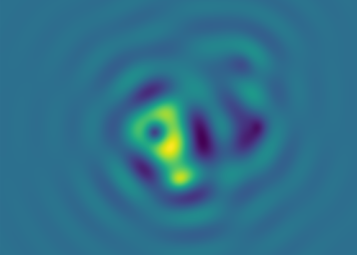
\includegraphics[width=.47\textwidth]{pictures/real_3d_part_projected}} &
        \subcaptionbox{\centering Imaginary part of $P \nabla G$ (the integrand) \label{fig:proj_b}}{
\includegraphics[width=.47\textwidth]{pictures/imag_3d_part_projected}} \\
        \subcaptionbox{\centering Real part of $P \nabla G$ (the integrand) at $x=0$ \label{fig:proj_c}}{\includegraphics[width=.47\textwidth]{pictures/real_2d_part}} &
        \subcaptionbox{\centering Imaginary part of $P \nabla G$ (the integrand) at $x=0$ \label{fig:proj_d}}{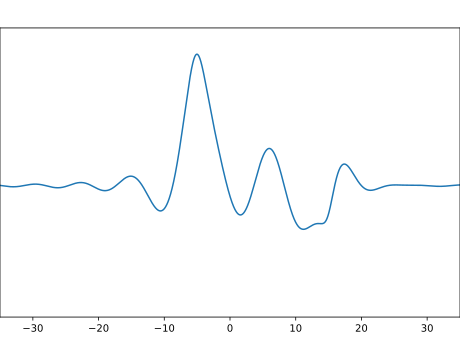
\includegraphics[width=.47\textwidth]{pictures/imag_2d_part}}
    \end{tabular}
    \caption{The integrand of the artificial Rayleigh integral for a prediction point at $(x_A, y_A, z_A) = (0.9, -1.4, -10)$ and sources at locations described in Section \ref{settings}. The Figures (a) and (b) are rotated such that the $y$-direction is horizontal and the $x$-direction is vertical. The Figures (c) and (d) can be extracted from Figures (a) and (b) by looking at the intensity of the wavefield in the middle, horizontal line (where $x=0$).}
    \label{fig:projected_wavefield}
\end{figure}
\begin{figure}[H]
    \vspace{-2em}
    \centering
    \begin{tabular}{cc}
        \subcaptionbox{\centering Real part of $P \nabla G$ (the integrand) at $x=0$ with 9 sample points, i.e. approximately 1.44 sample points per wavelength. \label{fig:samplesa}}{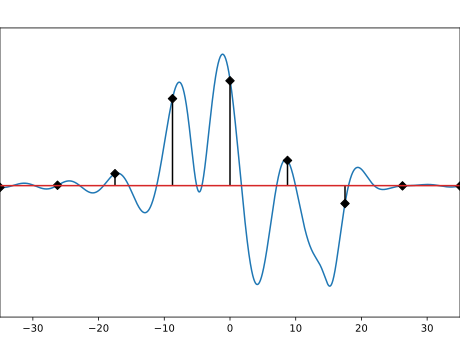
\includegraphics[width=.47\textwidth]{pictures/samples_19_9}} &
        \subcaptionbox{\centering Real part of $P \nabla G$ (the integrand) at $x=0$ with 29 sample points, i.e. approximately 5.03 sample points per wavelength.\label{fig:samplesb}}{\includegraphics[width=.47\textwidth]{pictures/samples_29_29}}
        % \subcaptionbox{\centering Real part of $P \nabla G$ (the integrand) at $x=0$ with 49 sample points, i.e. approximately 8.62 sample points per wavelength.\label{fig:samplesc}}{\includegraphics[width=.47\textwidth]{pictures/samples_49_49}} &
        % \subcaptionbox{\centering Real part of $P \nabla G$ (the integrand) at $x=0$ with 69 sample points, i.e. approximately 12.2 sample points per wavelength.\label{fig:samplesd}}{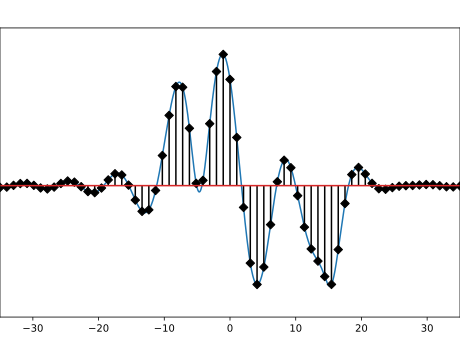
\includegraphics[width=.47\textwidth]{pictures/samples_69_69}}
    \end{tabular}
    \caption{Figure \ref{fig:proj_c}, displayed with varying amounts of sample points (per wavelength).}
\end{figure}

% Noise = 0.2\%, Max noise = 0.9\% for 500, Av noise = 0.16\%
\begin{table}[H]
\centering
    \begin{tabular}{|c|c|ccccccc|}
        \hline
        \multirow{2}{*}{Noise} & (points/$\lambda$)$_x$ & 4.52 & 7.04 & 12.1 & 17.1 & 24.6 & 49.8 & 125 \\
        & (points/$\lambda$)$_y$ & 1.44 & 5.03 & 8.62 & 12.2 & 17.6 & 35.5 & 89.4 \\
        % \multirow{2}{*}{Noise} & samples$_x$ & 19 & 29 & 49 & 69 & 99 & 199 & 499 \\
        % & samples$_y$ & 9 & 29 & 49 & 69 & 99 & 199 & 499 \\
        \hline
        \hline
        \rowcolor[gray]{.9}
        \cellcolor{white}
        & basic & 1.5 & 6.6$\cdot 10^{-3}$ & 1.1$\cdot 10^{-3}$ & 5.5$\cdot 10^{-4}$ & 2.7$\cdot 10^{-4}$ & 6.5$\cdot 10^{-5}$ & 1.0$\cdot 10^{-5 }$ \\
        \cline{2-9}
        \cellcolor{white}
        & combined & 1.60 & 0.305 & 0.298 & 0.827 & 7.06 & 406. & 63.5 \\
        \cellcolor{white}
        \multirow{-3}{*}{0\%}& separate & 1.03 & 1.88 & 4.21 & 28.0 & 44.8 & 183. & 1.14$\cdot 10^{3}$ \\
        \hline
        \hline
        \rowcolor[gray]{.9}
        \cellcolor{white}
        & basic & 1.5 & 6.6$\cdot 10^{-3}$ & 1.1$\cdot 10^{-3}$ & 4.7$\cdot 10^{-4}$ & 2.5$\cdot 10^{-4}$ & 6.0$\cdot10^{-5}$ & 1.0$\cdot 10^{-5 }$ \\
        \cline{2-9}
        \cellcolor{white}
        & basic$_\delta$ & 1.00 & 1.01 & 1.03 & 0.864 & 0.942 & 0.920 & 1.01 \\
        \cellcolor{white}
        & combined & 1.60 & 0.302 & 0.311 & 0.696 & 5.06 & 15.7 & 11.5 \\
        \cellcolor{white}
        & combined$_\delta$ & 1.60 & 0.301 & 0.322 & 0.638 & 3.65 & 46.2 & 3.71 \\
        \cellcolor{white}
        & separate & 1.03 & 1.89 & 5.05 & 17.4 & 20.8 & 8.82 & 16.4 \\
        \cellcolor{white}
        \multirow{-6}{*}{0.05\%}
        & separate$_\delta$ & 1.02 & 1.88 & 4.42 & 25.1 & 49.4 & 282. & 356. \\
        \hline
        \hline
        \rowcolor[gray]{.9}
        \cellcolor{white}
        & basic & 1.5 & 6.6$\cdot 10^{-3}$ & 1.3$\cdot 10^{-3}$ & 2.5$\cdot 10^{-4}$ & 2.0$\cdot 10^{-4}$ & 4.7$\cdot 10^{-5}$ & 1.1$\cdot 10^{-5 }$ \\
        \cline{2-9}
        \cellcolor{white}
        & basic$_\delta$ & 0.999 & 1.05 & 1.13 & 0.458 & 0.771 & 0.698 & 1.07 \\
        \cellcolor{white}
        & combined & 1.60 & 0.296 & 0.348 & 0.306 & 1.56 & 3.16 & 3.29 \\
        \cellcolor{white}
        & combined$_\delta$ & 1.61 & 0.296 & 0.404 & 0.242 & 1.25 & 9.89 & 0.996 \\
        \cellcolor{white}
        & separate & 1.02 & 1.90 & 7.32 & 1.77 & 4.72 & 1.76 & 4.29 \\
        \cellcolor{white}
        \multirow{-6}{*}{0.2\%}
        & separate$_\delta$ & 1.02 & 1.89 & 5.04 & 14.9 & 65.1 & 89.4 & 81.2 \\
        \hline
        \hline
        \rowcolor[gray]{.9}
        \cellcolor{white}
        & basic & 1.5 & 8.4$\cdot 10^{-3}$ & 2.1$\cdot 10^{-3}$ & 1.0$\cdot 10^{-3}$ & 1.6$\cdot 10^{-4}$ & 6.4$\cdot 10^{-5}$ & 2.1$\cdot 10^{-5 }$ \\
        \cline{2-9}
        \cellcolor{white}
        & basic$_\delta$ & 0.995 & 1.60 & 1.51 & 2.06 & 0.764 & 0.712 & 1.76 \\
        \cellcolor{white}
        & combined & 1.62 & 0.343 & 0.518 & 0.464 & 0.271 & 0.861 & 1.32 \\
        \cellcolor{white}
        & combined$_\delta$ & 1.64 & 0.339 & 1.36 & 0.361 & 0.251 & 2.79 & 0.390 \\
        \cellcolor{white}
        & separate & 1.01 & 1.67 & 2.75 & 1.36 & 0.783 & 0.479 & 1.69 \\
        \cellcolor{white}
        \multirow{-6}{*}{1\%}
        & separate$_\delta$ & 1.00 & 2.44 & 8.50 & 105. & 11.7 & 19.4 & 33.0 \\
        \hline
        \hline
        \rowcolor[gray]{.9}
        \cellcolor{white}
        & basic & 1.2 & 3.0$\cdot 10^{-2}$ & 6.2$\cdot 10^{-3}$ & 7.3$\cdot 10^{-3}$ & 1.6$\cdot 10^{-3}$ & 5.0$\cdot 10^{-4}$ & 9.4$\cdot 10^{-5 }$ \\
        \cline{2-9}
        \cellcolor{white}
        & basic$_\delta$ & 0.967 & 2.17 & 2.91 & 10.0 & 3.38 & 0.933 & 0.593 \\
        \cellcolor{white}
        & combined & 1.80 & 0.798 & 0.864 & 0.707 & 0.542 & 1.34 & 1.18 \\
        \cellcolor{white}
        & combined$_\delta$ & 1.90 & 0.788 & 0.900 & 0.587 & 0.507 & 4.38 & 0.333 \\
        \cellcolor{white}
        & separate & 0.925 & 1.46 & 1.39 & 1.94 & 1.60 & 0.754 & 1.54 \\
        \multirow{-6}{*}{5\%}
        \cellcolor{white}
        & separate$_\delta$ & 0.818 & 7.85 & 54.6 & 123. & 27.8 & 46.5 & 48.0 \\
        \hline
        \hline
        \rowcolor[gray]{.9}
        \cellcolor{white}
        & basic & 7.5$\cdot 10^{-2}$ & 1.3$\cdot 10^{-1}$ & 1.9$\cdot 10^{-2}$ & 3.0$\cdot 10^{-2}$ & 7.1$\cdot 10^{-3}$ & 2.2$\cdot 10^{-3}$ & 3.7$\cdot 10^{-4 }$ \\
        \cline{2-9}
        \cellcolor{white}
        & basic$_\delta$ & 0.548 & 1.40 & 1.56 & 3.70 & 0.898 & 0.302 & 0.147 \\
        \cellcolor{white}
        & combined & 0.129 & 1.19 & 1.11 & 0.765 & 0.588 & 1.40 & 1.18 \\
        \cellcolor{white}
        & combined$_\delta$ & 0.117 & 1.53 & 0.545 & 0.560 & 0.538 & 0.659 & 0.174 \\
        \cellcolor{white}
        & separate & 0.109 & 1.58 & 1.06 & 2.21 & 1.90 & 0.818 & 1.71 \\
        \cellcolor{white}
        \multirow{-6}{*}{20\%}
        & separate$_\delta$ & 0.0474 & 12.4 & 37.9 & 43.6 & 33.5 & 265. & 128. \\
        \hline
    \end{tabular}
    \caption{For different amounts of noise (normal distributed, with a standard deviation of 0\%, 0.05\%, 0.2\%, 1\%, 5\% and 20\% of the length between equidistant points) and different amounts of samples points per wavelength varying per direction ((4.52, 1.44), (7.04, 5.03), (12.1, 8.62), (17.1, 12.2), (24.6, 17.6), (49.8, 35.5), (125, 89.4)) we listed the relative error (the mean-squared error was used due to working with complex numbers) of the approximation of the simulated Rayleigh integral (with settings listed in Section \ref{settings}) using the basic method described in Section \ref{summary_used_method}.
    Also, the other methods described in Section \ref{summary_used_method} are listed (where the adapted version of the method on a non-equidistant grid is denoted with a subscript $\delta$) with their relative error, divided by the relative error of the basic method.
    We thus have that the numbers represent the number of times that the used method is better than the basic method.
    We note that for a noise of 0\% the adapted versions of each method are the same as the regular methods, since we have no uncertainty in gridpoints.
    Furthermore, to give an example: for a noise of 0.2\% (thus each gridpoints is shifted in the $x$-direction with $\mathcal N(0.2\% \cdot h_x)$ and in the $y$-direction with $\mathcal N(0.2\% \cdot h_y)$, where $h_x$, $h_y$ denote the distance between the equidistant gridpoints in the $x$ and $y$-directions respectively and $\mathcal N(\sigma)$ denotes normal distributed noise with standard deviation $\sigma$) and 12.1 samples per wavelength in the $x$-direction and $8.62$ samples per wavelength in the $y$-direction, the basic method has a relative error of $1.3\cdot 10^{-3}$, whereas the altered separate method (separate$_\delta$) has a relative error that is $5.04$ times as low, i.e. $1.3/5.04\cdot 10^{-3} \approx 2.6\cdot 10^{-4}$ and the combined method has a relative error that is larger than the error of the basic method with a factor of $1/0.348 \approx 2.87$.}
    \label{tab:single}
\end{table}


\begin{table}[H]
\centering
    \begin{tabular}{|c|c|ccccccc|}
        \hline
        \multirow{2}{*}{Noise} & (points/$\lambda$)$_x$ & 4.52 & 7.04 & 12.1 & 17.1 & 24.6 & 49.8 & 125 \\
        & (points/$\lambda$)$_y$ & 1.44 & 5.03 & 8.62 & 12.2 & 17.6 & 35.5 & 89.4 \\
        \hline
        \hline
        \rowcolor[gray]{.9}
        \cellcolor{white}
        & basic & 1.2 & 3.9$\cdot 10^{-3}$ & 1.2$\cdot 10^{-3}$ & 5.8$\cdot 10^{-4}$ & 2.8$\cdot 10^{-4}$ & 6.8$\cdot 10^{-5}$ & 1.1$\cdot 10^{-5 }$ \\
        \cline{2-9}
        \cellcolor{white}
        & combined & 1.51 & 0.173 & 0.323 & 3.31 & 13.5 & 219. & 62.0 \\
        \cellcolor{white}
        \multirow{-3}{*}{0\%}
        & separate & 1.01 & 1.01 & 13.0 & 63.3 & 104. & 433. & 2.66$\cdot 10^3$ \\
        \hline
        \hline
        \rowcolor[gray]{.9}
        \cellcolor{white}
        & basic & 1.2 & 3.9$\cdot 10^{-3}$ & 1.2$\cdot 10^{-3}$ & 5.4$\cdot 10^{-4}$ & 2.8$\cdot 10^{-4}$ & 6.6$\cdot 10^{-5}$ & 1.0$\cdot 10^{-5 }$ \\
        \cline{2-9}
        \cellcolor{white}
        & basic$_\delta$ & 1.00 & 1.02 & 1.01 & 0.932 & 0.985 & 0.958 & 0.953 \\
        \cellcolor{white}
        & combined & 1.51 & 0.173 & 0.321 & 2.30 & 5.41 & 19.8 & 9.10 \\
        \cellcolor{white}
        & combined$_\delta$ & 1.51 & 0.172 & 0.326 & 3.44 & 6.42 & 22.5 & 4.14 \\
        \cellcolor{white}
        & separate & 1.01 & 1.02 & 13.4 & 13.1 & 26.3 & 19.0 & 12.5 \\
        \cellcolor{white}
        \multirow{-6}{*}{0.05\%}
        & separate$_\delta$ & 1.01 & 1.01 & 14.0 & 76.0 & 136. & 890. & 1.22$\cdot 10^3$ \\
        \hline
        \hline
        \rowcolor[gray]{.9}
        \cellcolor{white}
        & basic & 1.1 & 4.1$\cdot 10^{-3}$ & 1.2$\cdot 10^{-3}$ & 4.8$\cdot 10^{-4}$ & 2.7$\cdot 10^{-4}$ & 6.0$\cdot 10 ^{-5}$ & 9.1$\cdot 10^{-6 }$ \\
        \cline{2-9}
        \cellcolor{white}
        & basic$_\delta$ & 1.00 & 1.07 & 1.03 & 0.845 & 0.955 & 0.869 & 0.886 \\
        \cellcolor{white}
        & combined & 1.51 & 0.176 & 0.315 & 1.78 & 1.88 & 5.05 & 2.30 \\
        \cellcolor{white}
        & combined$_\delta$ & 1.52 & 0.173 & 0.338 & 3.42 & 2.48 & 5.05 & 0.903 \\
        \cellcolor{white}
        & separate & 1.01 & 1.08 & 7.09 & 2.63 & 6.75 & 4.68 & 2.87 \\
        \cellcolor{white}
        \multirow{-6}{*}{0.2\%}
        & separate$_\delta$ & 1.01 & 1.05 & 18.7 & 130. & 265. & 159. & 188. \\
        \hline
        \hline
        \rowcolor[gray]{.9}
        \cellcolor{white}
        & basic & 1.1 & 5.9$\cdot 10^{-3}$ & 1.7$\cdot 10^{-3}$ & 1.2$\cdot 10^{-3}$ & 4.4$\cdot 10^{-4}$ & 6.5$\cdot 10 ^{-5}$ & 1.4$\cdot 10^{-5 }$ \\
        \cline{2-9}
        \cellcolor{white}
        & basic$_\delta$ & 0.999 & 1.52 & 1.40 & 2.74 & 2.25 & 1.15 & 1.58 \\
        \cellcolor{white}
        & combined & 1.52 & 0.229 & 0.409 & 0.808 & 0.733 & 1.18 & 0.832 \\
        \cellcolor{white}
        & combined$_\delta$ & 1.54 & 0.211 & 0.727 & 1.72 & 0.918 & 1.69 & 0.311 \\
        \cellcolor{white}
        & separate & 1.00 & 1.23 & 1.91 & 1.43 & 2.24 & 1.03 & 1.08 \\
        \cellcolor{white}
        \multirow{-6}{*}{1\%}
        & separate$_\delta$ & 0.993 & 1.50 & 16.4 & 62.1 & 58.1 & 27.6 & 48.1 \\
        \hline
        \hline
        \rowcolor[gray]{.9}
        \cellcolor{white}
        & basic & 9.3$\cdot 10^{-1}$ & 2.1$\cdot 10^{-2}$ & 5.2$\cdot 10^{-3}$ & 6.5$\cdot 10^{-3}$ & 1.9$\cdot 10^{-3}$ & 2.4$\cdot 10^{-4}$ & 8.6$\cdot 10^{-5 }$ \\
        \cline{2-9}
        \cellcolor{white}
        & basic$_\delta$ & 0.991 & 1.57 & 3.11 & 10.9 & 7.19 & 0.741 & 0.858 \\
        \cellcolor{white}
        & combined & 1.61 & 0.578 & 0.712 & 0.844 & 0.697 & 0.842 & 0.988 \\
        \cellcolor{white}
        & combined$_\delta$ & 1.73 & 0.457 & 1.82 & 1.74 & 0.799 & 1.76 & 0.369 \\
        \cellcolor{white}
        & separate & 0.936 & 1.37 & 1.09 & 1.60 & 1.98 & 0.628 & 1.24 \\
        \cellcolor{white}
        \multirow{-6}{*}{5\%}
        & separate$_\delta$ & 0.828 & 5.25 & 37.9 & 102. & 108. & 27.0 & 86.4 \\
        \hline
        \hline
        \rowcolor[gray]{.9}
        \cellcolor{white}
        & basic & 7.2$\cdot 10^{-2}$ & 9.0$\cdot 10^{-2}$ & 1.8$\cdot 10^{-2}$ & 2.7$\cdot 10^{-2}$ & 7.4$\cdot 10^{-3}$ & 1.1$\cdot 10^{-3}$ & 3.6$\cdot 10^{-4 }$ \\
        \cline{2-9}
        \cellcolor{white}
        & basic$_\delta$ & 0.886 & 1.16 & 3.94 & 3.89 & 1.04 & 0.224 & 0.223 \\
        \cellcolor{white}
        & combined & 0.159 & 1.00 & 0.884 & 0.858 & 0.694 & 0.923 & 1.04 \\
        \cellcolor{white}
        & combined$_\delta$ & 0.130 & 0.821 & 1.09 & 3.32 & 0.429 & 0.550 & 0.216 \\
        \cellcolor{white}
        & separate & 0.145 & 1.38 & 0.903 & 1.72 & 1.94 & 0.675 & 1.33 \\
        \cellcolor{white}
        \multirow{-6}{*}{20\%}
        & separate$_\delta$ & 0.0687 & 8.67 & 21.4 & 85.6 & 48.3 & 112. & 231. \\
        \hline
    \end{tabular}
    \caption{The average of Table \ref{tab:single} for the 10 prediction points listed in Section \ref{settings}. For further information on the meaning of the values the reader is referred to the caption of Table \ref{tab:single}.}
    \label{tab:average}
\end{table}

% Noise = 0.2\%, Max noise = 0.9\% for 500, Av noise = 0.16\%
Let us first have a look at Table \ref{tab:average}.
Note that the cells using the basic method have different units (relative error) than the cells using other methods (relative error/relative error = times better compared to basic method).

Generally, we expect that fewer points per wavelength result in higher relative errors and more noise also results in higher relative errors.
This relation does not hold in the first column (with 4.52, 1.44 points per wavelength) of the table as we go from a relative error in the basic method of $1.2$ at a noise of $0\%$ to a relative error of $7.2\cdot 10^{-2}$ at a noise of $20\%$.
This is most likely a coincidence (that did not smooth out in the average) as other methods did not have such sudden improvements.
If we go from 17.1, 12.2 sample points per wavelength to 12.1, 8.62 sample points per wavelength (thus from the fourth column to the third) and compare the relative errors in the basic methods with 5\% and 20\% noise, the error decreases.
Also, this effect is likely to be caused by chance, with such a high noise in the gridpoints the decrease in sample points does not outrank the coincidences caused by the noise.
All in all, we can see that apart from a few exceptions the relation holds (as expected).

The altered basic method (basic$_\delta$) performs better than the basic method with a noise of 1\% and not much worse for less noise.
However, for more noise (5\% and 20\%) and numerous points per wavelength it performs worse than the basic method.
This is probably due to the method not being exact for completely randomized grids, but only for rectilinear grids.
This limitation of the method combined with chance caused it to perform worse than the basic method.

If the integrand is well sampled and has a low amount of noise the combined method overtakes the basic method.
If noise increases the method is only a little worse than the basic method, likely due to inability to average the result as good as the basic method (it is more prone to errors and noise).
Since this method is relatively easy to implement it is recommended to use only with a noise below 1\% and more than 10 sample points per wavelength (in both directions).
If the noise increases, we can see no reason to choose this method over the basic method and if the number of sample points decreases we mainly have worse results.

The adaptation of the combined interpolation method (combined$_\delta$) often exceeds the regular combined method except for a large amount of sample points per wavelength.
Again, the reason for this is probably the fact that the randomized grid is not a semi-equidistant grid.
The trade-off for more operations hardly seems worth it.

The separate method performs really well with less noise and many sample points per wavelength, like the combined method.
This method, if compared to the combined method is generally better (except for the first column with the fewest sample points per wavelength).
Also, this method extends better to a low sample points per wavelength range (except the lowest).
The cost of using this method is that it is more difficult to implement and depending on the implementation (although it has the same time complexity as can be seen in Section \ref{summary_used_method}) it can take longer to compute the integral.

The final method, the modified separate method (separate$_\delta$), has the highest accuracy compared to all other described methods from the third column on (that is with more than 12.1, 8.62 sample points).
Especially with a high amount of noise (e.g. 1\%) this method really exceeds the others (by a factor of at least 15 if compared to the basic method).
This method also has peak performance with a lot of sample points per wavelength, but the remarkable thing is that with less sample points it still outperforms most of the other methods.
The cost of using this method is the implementation as it is the most difficult of all methods, nonetheless, the method makes up for this by accuracy.

Now, we provide a note on the time complexity of the methods from Section \ref{summary_used_method}.
The basic method, the altered basic method, the combined method and its modification all have the same time complexity (although for the alterations we do need more operations).
Compared to the separate methods the time complexity is better by a factor of $n_f m_f$ (the orders of the polynomials for the interpolation). This is, however, only true when using splines. In that case we need to process $n_f m_f$ coefficients per subinterval, compared to only 1 using combined methods.
If instead polynomials are used for this separate method (this is left to future research in Section \ref{discussion}) we get the same time complexity (apart from initialization costs, which can be neglected for many sensors).
The space complexity of the separate method does not have a serious limitation and is therefore only mentioned for completeness.


After comparing the values in Table \ref{tab:average} with Table \ref{tab:single} we can say something about the consistency of the method and see if there are outliers (remember that the former table took an average over multiple prediction points and the latter did not).

The basic method still has approximately the same error in this table.

Before the average was taken over multiple prediction points the basic$_\delta$ method is more unpredictable.
Therefore, we do not think it is worth the extra processing time.

Except for situations with noise below 0.2\% and more than 24.6, 17.6 sample points per wavelength in the $x$ and $y$-direction respectively the combined method is generally worse than the basic method.
We can also see this effect in Table \ref{tab:average}, although, the break-even point happened at 17.1, 12.2 sample points per wavelength, we thus conclude that this method cannot be relied upon for consistent results with moderate sampling amounts.

The adaptation of the combined method is also more unpredictable in this situation, instead of being (somewhat) consistently better than the unmodified method it is now at odds with it.

The separate method performed about the same, the numbers just varied more in Table \ref{tab:single}, whereas the sudden improvements were smoothed out in Table \ref{tab:average}.
The same effect occurred for the modified separate method, the factor that this method is better than the basic method does not always increase as the amount of sample points increase, nevertheless, the general trend is upward (since if we take the average we get the smoother version in Table \ref{tab:average}).

In conclusion:
\vspace{-.5em}
\begin{itemize}
    \itemsep0em
    \item The modified basic method is inconsistent.
    \item The combined method only performs well in the high sample points per wavelength range with hardly any noise.
    \item The adapted combined method is not worth the extra computation time compared to the original version.
    \item The separate method often performs better than the combined method and extends better to fewer sample points but takes more time to implement.
    \item The altered separate method performs the best, exceeding the performance of all other methods in most situations.
\end{itemize}

\chapter{Conclusion and outlook}
\label{conclusion}
\section{Conclusion}
% In this thesis we derived the Rayleigh integral and subsequently we used polynomial interpolation for numerical integration.
% Followed by modifying the integration methods to better fit the Rayleigh integral.
% The different methods used are
In this thesis we started with deriving the Rayleigh integral and subsequently developed polynomial interpolation methods for numerical integration in order to determine whether modifying the integration methods would reduce the error in approximations of the Rayleigh integral.
The presented methods are:
% in this these we started with deriving the ray integral and subsequently used poly interpolation for numerical integration in order to determine whether modyfing the integration methods would improve the fitting of the rayleigh integral.
% In this thesis we started with deriving the Rayleigh integral.
% Subsequently, we took a glance at using polynomial interpolation for numerical integration.
% Afterwards, we devoted a chapter to modifying the integration methods to better fit the Rayleigh integral, here we gave a quick overview of the presented methods:
\vspace{-.5em}
\begin{itemize}
    \itemsep0em
    \item The basic method; this is the one that is currently used for approximating the Rayleigh integral.
    \item An adaptation of the basic method; the basic method for a rectilinear grid.
    \item The combined interpolation method; Simpson's rule in our case.
    \item The modified combined interpolation method; an adaptation for a semi-equidistant grid.
    \item The separate interpolation method; this method separately interpolates the unknown part of the integrand (to a low degree) and the known part of the integrand (to a higher degree) and combines the results.
    \item The altered separate interpolation method; this is an adaptation of the separate interpolation method to non-equidistant grids.
\end{itemize}
\vspace{-.5em}
These different integration methods were then used to approximate a synthetic Rayleigh integral with varying amounts of noise in the sample points.
% In the final chapter we present the results of the different integration methods, that is, we approximate a synthetic Rayleigh integral (with varying amounts of noise in the sample points) using the different methods.

The best performing method is the altered version of the separate interpolation method. It outperforms all other methods in accuracy and is on average, in comparison with the currently used method, at least 15 times better in the moderate to well sampled range\footnote{This is the achieved with more than 12 sample points per wavelength in the $x$-direction and more than 8 sample points per wavelength in the $y$-direction.}.

Our adjustment to the basic method only performed marginally better and the cost of more operations is not beneficial.

The combined interpolation approach performed well with relatively small noise (up to about 1\% of the distance between gridpoints) and more than 10 sample points per wavelength (in both directions). However, the improvement on the approximation fluctuates too much to be relied upon if the conditions are not met. An advantage of this method is that it is relatively easy to implement.

The modified version of the method also has a lot of fluctuations, giving inconsistent results that are on average only marginally better than the original version. Therefore, we do not think that the extra computation time is worth it in comparison to the combined method.

The separate interpolation method scores only slightly better than the combined method, it had peak-performance with almost no noise and numerous sample points per wavelength. However, this method is more difficult to implement and will likely take longer to evaluate than the combined method, hence, this method is not recommended.



\section{Future Research}
\label{discussion}
In future research we recommend to look at making an ``accuracy vs speed'' analysis.
In seismic imaging it is crucial that the first propagations of the wavefield are accurate, if the error in these propagations are too large one has no hope to arrive at a decent answer after propagating it hundreds of times more.
Since we presented methods to increase accuracy a researcher could look at using different methods for different propagations, to get a better result in the first few propagations and to limit the error in the end result.
Our presented methods likely take more time to evaluate, therefore, an optimum can be found if we compare accuracy to speed and use various methods.

Placing the sensors is important, the methods presented could yield better results if the grid is not placed approximately equidistant, i.e. some the methods could perform better on a different grid. An example of this could be a triangular grid, which could also result in time advantages using the modified separate interpolation method as this relies on triangulating the input data. In addition, one could look at systematic errors in gridpoints and the impact of those on the accuracy of the different methods.

Also, an implementation of some algorithms would be needed to perform a speed analysis of the methods.
Even though the time complexity of the algorithms is the same, it depends on the computer used and the implementation of the method.

Another combined interpolation method of using higher-order polynomials was discussed shortly in this thesis.
The methods were not developed further because of great deflections on the boundaries of the interpolation.
In Section \ref{examples} we provided a way to circumvent this problem, giving adequate results in that example.
For these methods there are a lot of possible variations, as one could go to arbitrary orders of polynomials.
In future research one could look at the accuracy of those methods as they would be easy to implement.

The separate interpolation method could also be made easier to implement by using polynomial interpolation instead of spline interpolation.
We did not compute the results for this new method.
This would promote the separate interpolation even more as the downside of difficult implementations would reduce.

% \input{todo}
% \input{no_use}

\appendix
% \chapter{Begin Stream}
\chapter{Verification of the wave equation}
\label{appendix:wave_eq}

\begin{wrapfigure}{r}{.4\textwidth}
    \vspace{-12pt}
    \centering
    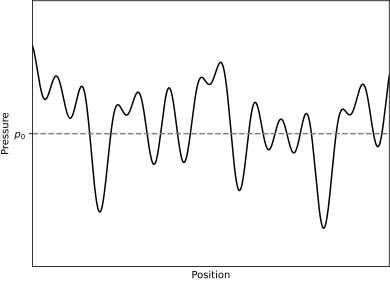
\includegraphics[width=.4\textwidth]{pictures/random_pressure}
    % \captionsetup{justification=centering}
    \vspace{-1.5em}
    \caption{Some function of pressure depending on position that will change with time.}
    \label{fig:pres_pos}
    \vspace{-1.5em}
\end{wrapfigure}

This is an intuitive verification of the one-dimensional acoustic wave equation\footnote{Notation and ideas used in this appendix are adapted from \citeauthor{notation_intuitive} \cite{notation_intuitive}.} (the three-dimensional version is derived in Section \ref{sec:wave_eq}).
To start off with this approach, let us assume that there is no sound.
Then, no vibrations in the air can occur which, in turn, results in equal pressure in the air not varying with position (denoted $p_0$).

However, if there is sound we do get vibrations and therefore some variation of pressure depending on the position you are measuring the sound as can be seen in Figure \ref{fig:pres_pos}.

To gain intuition for what happens over time let us discretize the pressure function and pick only 3 ``adjacent'' points from the function.
This can also be thought of as zooming in on Figure \ref{fig:pres_pos} until you see only 3 points.
An example of this can be seen in Figure \ref{fig:zoom_1}.
We take look at how the pressure of the middle point, $p_2$, changes as a function of its differences with $p_1$ and $p_3$. After rewriting this function we look at the limit and get the partial differential equation named the one-dimensional acoustic wave equation.

So, to begin we start at $t=0$ with Figure \ref{fig:zoom_1}, the three points are denoted $x_1$, $x_2$, and $x_3$ with corresponding pressures $p_1$, $p_2$, and $p_3$, respectively.
We assume that $p_1$ and $p_3$ are fixed and investigate the function $p_2$ describes (note that the values $1$ for $p_1$, $4$ for $p_2$ and $-1$ for $p_3$ are chosen arbitrarily and can be scaled appropriately).
We start with the situation where the air at $x_1$, $x_2$, and $x_3$ has no velocity.
Because there is a high pressure at $x_2$ and lower pressures at $x_1$ and $x_3$, the system wants to ``equalize'' the pressure, and we get a large acceleration of air from $x_2$ towards $x_1$ and $x_3$ (from now on we say that $p_2$ has a large acceleration towards $p_0$, the static pressure), but since the system needs time to ``start up'' the velocity of the individual particles stays small but will increase rapidly. The total change in pressure will thus be little, giving the situation in Figure \ref{fig:zoom_2}.

Now the velocity of the individual particles, i.e. the change in pressure, has started to build up, although the acceleration of $p_2$ towards $p_0$ has started to decrease due to the decreased difference to $p_1$ and $p_3$ (the system does not want to ``equalize'' the pressure as much) thus the velocity of $p_2$ towards $p_0$ will not increase as much as last time. We obtain the situation in Figure \ref{fig:zoom_3}.

The velocity still increases due to a positive acceleration but with each timestep the acceleration decreases. Hence, the velocity will increase less and less, resulting in the situation in Figure \ref{fig:zoom_4}.

At this point we have $p_1=p_2$ meaning that $x_1$ and $x_2$ are in equilibrium, however, $x_2$ and $x_3$ are not. So there will still be a positive acceleration, due to a high velocity, the pressure in $x_2$, $p_2$, shoots past the static pressure $p_0$. At the next timestep we see something like the situation in Figure \ref{fig:zoom_5}.

The velocity starts to decrease because of the difference in pressure at $x_1$ and $x_2$, thus we have negative acceleration. But the velocity is still positive thus we still get a decreasing pressure in $x_2$. Due to the negative acceleration that keeps on increasing as $p_3$ decreases, the velocity will eventually be 0 again. This happens in the situation in Figure \ref{fig:zoom_6}, at $t=7$.

\begin{figure}[h]
    % \vspace{-10pt}
    \begin{tabular}{cccc}
        \subcaptionbox{\centering Situation at $t=0$\label{fig:zoom_1}}{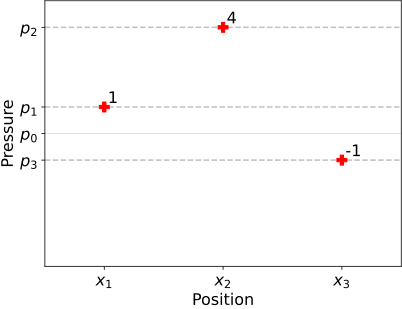
\includegraphics[width=.3\textwidth]{pictures/pressure_zoom_1}} &
        \subcaptionbox{\centering Situation at $t=1$\label{fig:zoom_2}}{\includegraphics[width=.3\textwidth]{pictures/pressure_zoom_2}} &
        \subcaptionbox{\centering Situation at $t=2$\label{fig:zoom_3}}{\includegraphics[width=.3\textwidth]{pictures/pressure_zoom_3}} \\
        \subcaptionbox{\centering Situation at $t=3$\label{fig:zoom_4}}{\includegraphics[width=.3\textwidth]{pictures/pressure_zoom_4}} &
        \subcaptionbox{\centering Situation at $t=4$\label{fig:zoom_5}}{\includegraphics[width=.3\textwidth]{pictures/pressure_zoom_5}} &
        \subcaptionbox{\centering Situation at $t=7$\label{fig:zoom_6}}{\includegraphics[width=.3\textwidth]{pictures/pressure_zoom_6}} &
    \end{tabular}
    \caption{Zoomed in version of Figure \ref{fig:pres_pos}, here $p_1=p(x_1)$, $p_2=p(x_2)$ and $p_3=p(x_3)$. Note that the timesteps can be scaled appropriately.}
\end{figure}

We have gotten a more intuitive feel of how the differences in pressure increase the acceleration of the pressure. To put that thought in formulas, we get that the acceleration of the pressure (its 2nd time derivative) is a function of the sum of differences between $p_1$ and $p_2$ and between $p_2$ and $p_3$, thus after defining some constant $\alpha$ and noting that positive acceleration defined is upwards we get (note that $\Delta$ denotes the spatial difference):
\begin{equation}
    \frac{\partial^2 p}{\partial t^2} = -\alpha (\underbrace{(p_2-p_1)}_{\Delta p_1} + \underbrace{(p_2-p_3)}_{-\Delta p_2}) = \alpha \underbrace{(\Delta p_2 - \Delta p_1)}_{\Delta\Delta p_1} \,.\label{eq:dif_of_dif}
\end{equation}
Thus, $\frac{\partial^2 p}{\partial t^2}$ is a function of the spatial difference of $\Delta p_1$ and $\Delta p_2$, thus it can be denoted by the second spatial difference $\Delta \Delta p_1$.
Now, if we take the limit so that the difference in positions goes to zero ($(x_2-x_1) \to 0$ and $(x_3-x_2) \to 0$ as well). We get that these differences turn into spatial derivates. Then \ref{eq:dif_of_dif} becomes
\begin{equation}
    \frac{\partial^2 p}{\partial t^2} = \alpha \frac{\partial^2 p}{\partial x^2}\,, \nonumber
\end{equation}
which is the one-dimensional acoustic wave equation.

\input{appendix-b}
\chapter{Matrices from the example calculation}
\label{app:B}


%%% THIS IS WITHOUT SHIFTING
% \begin{align}
%     b_{ij} &= \begin{bmatrix}
%         0.68896 & 0.4346 & -0.02944 & -0.0097228 \\
%         0.68896 & 0.4346 & -0.02944 & -0.0097228 \\
%         0.42002 & 0.16566 & -0.11909 & -0.019683 \\
%         0.43745 & 0.20053 & -0.095841 & -0.014518 \\
%         0.43745 & 0.20053 & -0.095841 & -0.0025022 \\
%         0.39041 & 0.29461 & -0.15856 & 0.011436 \\
%         0.21126 & 0.47376 & -0.21828 & 0.018071 \\
%         0.21126 & 0.47376 & -0.21828 & 0.018071
%     \end{bmatrix} \,, \nonumber \\
%     c_{ik} &= \begin{bmatrix}
%         0.90797 & -0.12475 & -0.074376 & 0.018042 & 0.0044396 & 0.00021437 \\
%         1.0044 & -0.026695 & -0.034541 & 0.026119 & 0.0052566 & 0.00024732 \\
%         0.98878 & -0.052314 & -0.051575 & 0.020379 & 0.0042759 & 0.0001794 \\
%         0.98777 & -0.055127 & -0.054793 & 0.018459 & 0.003669 & 9.6965e-05 \\
%         0.98777 & -0.055268 & -0.053976 & 0.016086 & 0.0059934 & -0.001363 \\
%         0.89761 & 0.18189 & -0.30059 & 0.14164 & -0.024691 & 0.0013866 \\
%         1.547 & -0.76555 & 0.24232 & -0.009532 & -0.0046052 & 0.00040516 \\
%         2.204 & -1.5504 & 0.61913 & -0.10037 & 0.0063825 & -0.00012811
%     \end{bmatrix}\,.\nonumber
% \end{align}
% Therefore we can calculate $d_{ij}$

% \begin{equation}
%     d_{ij} &= \begin{bmatrix}
%         -0.85182 & 4.581 & -24.779 & 134.77 \\
%         0.14203 & -0.40212 & 1.0446 & -2.2333 \\
%         1.0466 & -2.2663 & 5.0931 & -11.85 \\
%         1.4641 & -1.0826 & 1.0714 & -1.1961 \\
%         1.3856 & 1.0132 & 1.0001 & 1.1164 \\
%         1.2855 & 2.9006 & 6.7888 & 16.416 \\
%         1.4454 & 5.4406 & 20.747 & 80.113 \\
%         1.3892 & 7.2533 & 38.127 & 201.75
%     \end{bmatrix}\,.\nonumber
% \end{equation}


% \section{Matrices $b_{ij}$, $c_{ij}$ and $d_{ij}$}
\label{app:matrices}
These are the matrices from the example calculation in Section \ref{examples} for the separate interpolation method described in Section \ref{sep_interpol}.
The computer code for generating these matrices can be found in Appendix \ref{app:code}.

\vfill
\vfill
\vfill
\begin{equation}
    B = \begin{bmatrix}
        -0.87832 & -0.26219 & 0.14557 & -0.0097228 \\
        -0.97689 & 0.10889 & 0.10182 & -0.0097228 \\
        -0.61727 & 0.34872 & 0.058066 & -0.019683 \\
        -0.02998 & 0.39005 & -0.03051 & -0.014518 \\
        0.43745 & 0.20053 & -0.095841 & -0.0025022 \\
        0.51415 & -0.10389 & -0.1071 & 0.011436 \\
        0.15594 & -0.348 & -0.055639 & 0.018071 \\
        -0.43025 & -0.39293 & 0.025681 & 0.018071
    \end{bmatrix} \,, \nonumber
\end{equation}
\vfill
\begin{equation}
    C = \begin{bmatrix}
        -0.83134 & 0.26959 & 0.096787 & -0.011336 & -0.0019914 & 0.00021437 \\
        -0.2559 & 0.46198 & 0.026152 & -0.018416 & -0.00030821 & 0.00024732 \\
        0.43407 & 0.41822 & -0.052521 & -0.014786 & 0.0015849 & 0.0001794 \\
        0.90271 & 0.18678 & -0.091602 & -0.0013727 & 0.0029417 & 0.000096965 \\
        0.98777 & -0.055268 & -0.053976 & 0.016086 & 0.0059934 & -0.001363 \\
        0.85769 & -0.062041 & 0.05026 & 0.024694 & -0.014291 & 0.0013866 \\
        0.89925 & 0.097732 & 0.017243 & -0.028331 & 0.0014721 & 0.00040516 \\
        0.99955 & -0.011708 & -0.077081 & -0.011424 & 0.0035001 & -0.00012811
    \end{bmatrix}\,,\nonumber
\end{equation}
\vfill
\begin{equation}
    D = \begin{bmatrix}
        -0.8518 & -0.52995 & -0.47276 & -0.49211 \\
        0.14199 & 0.23699 & 0.3016 & 0.38253 \\
        1.0466 & 0.87334 & 0.91425 & 1.0546 \\
        1.4641 & 1.1135 & 1.1177 & 1.2588 \\
        1.3856 & 1.0132 & 1.0001 & 1.1164 \\
        1.2855 & 0.97247 & 0.97915 & 1.1071 \\
        1.4454 & 1.1042 & 1.1126 & 1.2566 \\
        1.3901 & 1.0027 & 0.97905 & 1.0837
    \end{bmatrix}\,.\nonumber
\end{equation}
\vfill
\vfill
\vfill

\chapter{Computer code}
\label{app:code}
This computer code is for the example calculation conducted in Section \ref{examples}.
The implemented method is from Section \ref{sep_interpol} and can function as a guideline for future research.
\inputpython{scripts/example_calculation_separate_clean.py}
This is the computer code for generating the results from Chapter \ref{chap5}.
\inputpython{scripts/3d_visualizing.py}


{
    \emergencystretch=3em
    \hypersetup{citecolor=black, urlcolor=black, linkcolor=black}
    \printbibliography[heading=bibintoc]
}

\clearpage
\vspace*{\fill}
\hfill
\begin{center}
% \textsl{This page would be intentionally left blank if we would not wish to inform about that.}
\textsl{This page intentionally left blank.}

\vspace{2em}

\footnotesize{(in order to achieve a total page count of 73; a prime number)}
\end{center}
\vspace{\fill}
\thispagestyle{empty}
\newpage
\if@twocolumn\hbox{}\newpage\fi

\end{document}
